% Options for packages loaded elsewhere
\PassOptionsToPackage{unicode}{hyperref}
\PassOptionsToPackage{hyphens}{url}
%
\documentclass[
  9pt,
  ignorenonframetext,
]{beamer}
\usepackage{pgfpages}
\setbeamertemplate{caption}[numbered]
\setbeamertemplate{caption label separator}{: }
\setbeamercolor{caption name}{fg=normal text.fg}
\beamertemplatenavigationsymbolsempty
% Prevent slide breaks in the middle of a paragraph
\widowpenalties 1 10000
\raggedbottom
\setbeamertemplate{part page}{
  \centering
  \begin{beamercolorbox}[sep=16pt,center]{part title}
    \usebeamerfont{part title}\insertpart\par
  \end{beamercolorbox}
}
\setbeamertemplate{section page}{
  \centering
  \begin{beamercolorbox}[sep=12pt,center]{part title}
    \usebeamerfont{section title}\insertsection\par
  \end{beamercolorbox}
}
\setbeamertemplate{subsection page}{
  \centering
  \begin{beamercolorbox}[sep=8pt,center]{part title}
    \usebeamerfont{subsection title}\insertsubsection\par
  \end{beamercolorbox}
}
\AtBeginPart{
  \frame{\partpage}
}
\AtBeginSection{
  \ifbibliography
  \else
    \frame{\sectionpage}
  \fi
}
\AtBeginSubsection{
  \frame{\subsectionpage}
}
\usepackage{lmodern}
\usepackage{amssymb,amsmath}
\usepackage{ifxetex,ifluatex}
\ifnum 0\ifxetex 1\fi\ifluatex 1\fi=0 % if pdftex
  \usepackage[T1]{fontenc}
  \usepackage[utf8]{inputenc}
  \usepackage{textcomp} % provide euro and other symbols
\else % if luatex or xetex
  \usepackage{unicode-math}
  \defaultfontfeatures{Scale=MatchLowercase}
  \defaultfontfeatures[\rmfamily]{Ligatures=TeX,Scale=1}
\fi
\usetheme[]{Boadilla}
\usecolortheme{seahorse}
% Use upquote if available, for straight quotes in verbatim environments
\IfFileExists{upquote.sty}{\usepackage{upquote}}{}
\IfFileExists{microtype.sty}{% use microtype if available
  \usepackage[]{microtype}
  \UseMicrotypeSet[protrusion]{basicmath} % disable protrusion for tt fonts
}{}
\makeatletter
\@ifundefined{KOMAClassName}{% if non-KOMA class
  \IfFileExists{parskip.sty}{%
    \usepackage{parskip}
  }{% else
    \setlength{\parindent}{0pt}
    \setlength{\parskip}{6pt plus 2pt minus 1pt}}
}{% if KOMA class
  \KOMAoptions{parskip=half}}
\makeatother
\usepackage{xcolor}
\IfFileExists{xurl.sty}{\usepackage{xurl}}{} % add URL line breaks if available
\IfFileExists{bookmark.sty}{\usepackage{bookmark}}{\usepackage{hyperref}}
\hypersetup{
  pdftitle={Master en Big Data. Fundamentos matemáticos del análisis de datos.},
  pdfauthor={Fernando San Segundo},
  hidelinks,
  pdfcreator={LaTeX via pandoc}}
\urlstyle{same} % disable monospaced font for URLs
\newif\ifbibliography
\usepackage{color}
\usepackage{fancyvrb}
\newcommand{\VerbBar}{|}
\newcommand{\VERB}{\Verb[commandchars=\\\{\}]}
\DefineVerbatimEnvironment{Highlighting}{Verbatim}{commandchars=\\\{\}}
% Add ',fontsize=\small' for more characters per line
\usepackage{framed}
\definecolor{shadecolor}{RGB}{248,248,248}
\newenvironment{Shaded}{\begin{snugshade}}{\end{snugshade}}
\newcommand{\AlertTok}[1]{\textcolor[rgb]{0.94,0.16,0.16}{#1}}
\newcommand{\AnnotationTok}[1]{\textcolor[rgb]{0.56,0.35,0.01}{\textbf{\textit{#1}}}}
\newcommand{\AttributeTok}[1]{\textcolor[rgb]{0.77,0.63,0.00}{#1}}
\newcommand{\BaseNTok}[1]{\textcolor[rgb]{0.00,0.00,0.81}{#1}}
\newcommand{\BuiltInTok}[1]{#1}
\newcommand{\CharTok}[1]{\textcolor[rgb]{0.31,0.60,0.02}{#1}}
\newcommand{\CommentTok}[1]{\textcolor[rgb]{0.56,0.35,0.01}{\textit{#1}}}
\newcommand{\CommentVarTok}[1]{\textcolor[rgb]{0.56,0.35,0.01}{\textbf{\textit{#1}}}}
\newcommand{\ConstantTok}[1]{\textcolor[rgb]{0.00,0.00,0.00}{#1}}
\newcommand{\ControlFlowTok}[1]{\textcolor[rgb]{0.13,0.29,0.53}{\textbf{#1}}}
\newcommand{\DataTypeTok}[1]{\textcolor[rgb]{0.13,0.29,0.53}{#1}}
\newcommand{\DecValTok}[1]{\textcolor[rgb]{0.00,0.00,0.81}{#1}}
\newcommand{\DocumentationTok}[1]{\textcolor[rgb]{0.56,0.35,0.01}{\textbf{\textit{#1}}}}
\newcommand{\ErrorTok}[1]{\textcolor[rgb]{0.64,0.00,0.00}{\textbf{#1}}}
\newcommand{\ExtensionTok}[1]{#1}
\newcommand{\FloatTok}[1]{\textcolor[rgb]{0.00,0.00,0.81}{#1}}
\newcommand{\FunctionTok}[1]{\textcolor[rgb]{0.00,0.00,0.00}{#1}}
\newcommand{\ImportTok}[1]{#1}
\newcommand{\InformationTok}[1]{\textcolor[rgb]{0.56,0.35,0.01}{\textbf{\textit{#1}}}}
\newcommand{\KeywordTok}[1]{\textcolor[rgb]{0.13,0.29,0.53}{\textbf{#1}}}
\newcommand{\NormalTok}[1]{#1}
\newcommand{\OperatorTok}[1]{\textcolor[rgb]{0.81,0.36,0.00}{\textbf{#1}}}
\newcommand{\OtherTok}[1]{\textcolor[rgb]{0.56,0.35,0.01}{#1}}
\newcommand{\PreprocessorTok}[1]{\textcolor[rgb]{0.56,0.35,0.01}{\textit{#1}}}
\newcommand{\RegionMarkerTok}[1]{#1}
\newcommand{\SpecialCharTok}[1]{\textcolor[rgb]{0.00,0.00,0.00}{#1}}
\newcommand{\SpecialStringTok}[1]{\textcolor[rgb]{0.31,0.60,0.02}{#1}}
\newcommand{\StringTok}[1]{\textcolor[rgb]{0.31,0.60,0.02}{#1}}
\newcommand{\VariableTok}[1]{\textcolor[rgb]{0.00,0.00,0.00}{#1}}
\newcommand{\VerbatimStringTok}[1]{\textcolor[rgb]{0.31,0.60,0.02}{#1}}
\newcommand{\WarningTok}[1]{\textcolor[rgb]{0.56,0.35,0.01}{\textbf{\textit{#1}}}}
\usepackage{graphicx,grffile}
\makeatletter
\def\maxwidth{\ifdim\Gin@nat@width>\linewidth\linewidth\else\Gin@nat@width\fi}
\def\maxheight{\ifdim\Gin@nat@height>\textheight\textheight\else\Gin@nat@height\fi}
\makeatother
% Scale images if necessary, so that they will not overflow the page
% margins by default, and it is still possible to overwrite the defaults
% using explicit options in \includegraphics[width, height, ...]{}
\setkeys{Gin}{width=\maxwidth,height=\maxheight,keepaspectratio}
% Set default figure placement to htbp
\makeatletter
\def\fps@figure{htbp}
\makeatother
\setlength{\emergencystretch}{3em} % prevent overfull lines
\providecommand{\tightlist}{%
  \setlength{\itemsep}{0pt}\setlength{\parskip}{0pt}}
\setcounter{secnumdepth}{-\maxdimen} % remove section numbering
% Adaptado de http://rmarkdown.rstudio.com/articles_beamer.html

\usepackage[spanish, es-tabla, es-nodecimaldot]{babel}

%\usepackage{multirow}
%\usepackage{graphicx}
%\usepackage{rotating}
%\setbeamertemplate{caption}[numbered]
%\usepackage{hyperref}
%\usepackage{caption}
%\usepackage[normalem]{ulem}
%	\mode<presentation>
%\usepackage{wasysym}
\usepackage{amsmath}
%\usepackage{array}
%\usetheme{Warsaw}
%\usecolortheme{spruce}
%\usepackage{attachfile}
%\usepackage[dvipsnames]{xcolor}
%\definecolor{DarkGreen}{HTML}{009900}



\AtBeginSection{\frame{\sectionpage}}
\AtBeginSubsection{\frame{\subsectionpage}}
\newtranslation[to=spanish]{Section}{Secci\'on}
\newtranslation[to=spanish]{Subsection}{Subsecci\'on}

\usepackage{keystroke}


% logo of my university
\titlegraphic{
\includegraphics[width=4cm]{../fig/logoDMAsmall.png}}

\newcommand{\link}[2]{\textcolor{blue}{{\href{#1}{#2}}}}

\definecolor{Gris050}{gray}{0.50}
\definecolor{Gris025}{gray}{0.75}
\definecolor{Gris010}{gray}{0.90}

\title{Master en Big Data. Fundamentos matemáticos del análisis de datos.}
\subtitle{Tema 5: Introducción a la Inferencia Estadística.}
\author{Fernando San Segundo}
\date{Curso 2019-20. Última actualización: 2019-09-19}

\begin{document}
\frame{\titlepage}

%\tableofcontents

\begin{frame}
  \tableofcontents[hideallsubsections]
\end{frame}
\hypertarget{el-teorema-central-del-limite.}{%
\section{El Teorema Central del
Límite.}\label{el-teorema-central-del-limite.}}

\begin{frame}{Medias muestrales.}
\protect\hypertarget{medias-muestrales.}{}

\begin{itemize}
\item
  En temas anteriores hemos visto de manera informal y mediante
  simulaciones que la distribución muestral de la media producía una
  curva normal. Ahora que sabemos más sobre la normal vamos a expresar
  ese resultado de forma más precisa y lo usaremos para empezar a hacer
  Inferencia.
\item
  Queremos estudiar la distribución de una variable aleatoria
  cuantitativa \(X\) definida en los individuos de cierta población. En
  particular, la variable \(X\) tendrá una media \(\mu\) y una varianza
  \(\sigma^2\). 
\item
  Vamos a \textbf{estimar} el valor de \(\mu\) usando \textbf{muestras}
  de la población. Si tenemos una \textbf{muestra aleatoria simple}
  formada por \(n\) valores como \(x_1,\, x_2,\,\ldots,\, x_n\)
  (elegidos al azar y con remplazamiento) podemos usar la media muestral
  \[
  \bar x = \dfrac{x_1 + x_2 + \cdots + x_n}{n}
  \] para estimar la media poblacional \(\mu\).
\end{itemize}

\end{frame}

\begin{frame}{El espacio muestral.}
\protect\hypertarget{el-espacio-muestral.}{}

\begin{itemize}
\item
  Es el conjunto de todas las muestras aleatorias simples posibles de
  tamaño \(n\) que llamaremos \(\Omega^n\). Como ya vimos, al pasar de
  la población original al espacio muestral en general estamos pasando a
  un espacio muchísimo más grande.
\item
  \textbf{Ejemplo:} si tenemos una población de tamaño \(1000\),
  ¿cuántas muestras aleatorias simples de tamaño 7 podemos construir? Es
  fácil ver que son \[1000^7 = 1000000000000000000000\] muestras
  distintas.
\item
  Entre todas esas muestras hay \emph{muestras buenas} (en las que
  \(\bar x\approx\mu\)) y \emph{muestras malas}, con un valor de
  \(\bar x\) poco representativo. Si elegimos la muestra al azar,
  \emph{¿cómo de probable es que nos toque una muestra buena?}
\item
  Para responder necesitamos información sobre la distribución de los
  valores de \(\bar X\) entre todas las muestras posibles (en
  \(\Omega^n\)).
\end{itemize}

\end{frame}

\begin{frame}{Distribución muestral de la media: teorema central del
límite (TCL).}
\protect\hypertarget{distribucion-muestral-de-la-media-teorema-central-del-limite-tcl.}{}

\begin{itemize}
\tightlist
\item
  Sea \(X\) una v.a. con media \(\mu_X\) y varianza \(\sigma^2\). Sea
  \(\bar X\) la media muestral construida a partir de una muestra
  aleatoria simple \(X_1, X_2,\cdots, X_n\) de tamaño \(n\). Es decir:
  \[\bar X = \dfrac{X_1+X_2+\cdots +X_n}{n}\] donde las \(X_i\) son
  \emph{copias independientes entre sí de \(X\)}.
\end{itemize}

\begin{center}
  \fcolorbox{black}{Gris025}{\begin{minipage}{10cm}
  Teorema Central del Límite.\\
  Cuando consideramos valores {\bf suficientemente grandes} del tamaño muestral $n$, la distribución de la media muestral en el espacio muestral $\Omega^n$ se aproxima a una variable normal, cuya media y varianza son:
$$
\bar X \sim N\left(\mu_X,\frac{\sigma}{\sqrt{n}}\right) \qquad
$$
\end{minipage}}
\end{center}

\begin{itemize}
\tightlist
\item
  ¿Cuánto es \emph{suficientemente grande}? Depende de la población
  inicial. Por ejemplo, si la población es normal, \(n\) puede ser
  arbitrariamente pequeño (incluso \(n = 1\)). Pero si la población es,
  por ejemplo, muy asimétrica, entonces puede que necesitemos \(n\)
  bastante grande.
\end{itemize}

\end{frame}

\hypertarget{intervalos-de-confianza-para-la-media.}{%
\section{Intervalos de confianza para la
media.}\label{intervalos-de-confianza-para-la-media.}}

\begin{frame}{Estimación en forma de intervalo.}
\protect\hypertarget{estimacion-en-forma-de-intervalo.}{}

\begin{itemize}
\item
  Empezamos pensando en el caso más sencillo: suponemos que la variable
  \(X\) es (aproximadamente) normal, pero desconocemos su media \(\mu\)
  y queremos estimarla usando muestras.
\item
  Este caso es bastante frecuente porque hay muchas magnitudes en la
  naturaleza cuya distribución es (aproximadamente) normal.
\item
  Si \(X\) es normal el TCL es válido para cualquier tamaño muestral
  \(n\). Podemos tomar una muestra aleatoria simple y usar la estimación
  \(\mu\approx\bar X\). Naturalmente esto significa; \[
  \mu = \bar X + \text{error}
  \] Es muy importante entender que \textbf{el error es aleatorio}.
\item
  Para que esto tenga alguna utilidad científica es imprescindible
  cuantificar ese error. Si descubrimos que el tamaño del error es menor
  que \(\delta\) (piensa en un número pequeño) entonces podremos decir
  que: \[
  \bar X - \delta < \mu < \bar X + \delta
  \] y nuestra estimación de \(\mu\) será \textbf{en forma de intervalo}
  \((a, b) = (\bar X - \delta, \bar X + \delta)\). Como veremos el TCL
  nos ayuda a (obtener \(\delta\) y) construir esos intervalos.
\end{itemize}

\end{frame}

\begin{frame}[fragile]{El error es aleatorio porque la muestra es
aleatoria.}
\protect\hypertarget{el-error-es-aleatorio-porque-la-muestra-es-aleatoria.}{}

\begin{itemize}
\item
  En esta figura (mira el código que la ha generado) hemos obtenido 20
  muestras de tamaño \(n = 30\). La marca roja indica la media de la
  población, que es \(\mu =0\). Los puntos de cada muestra (puntos
  azules) están todos a la misma altura y se señala la media de esa
  muestra con un rombo naranja. Como ves, el error es aleatorio.
  Recuerda que en un caso real no sabemos donde está la línea roja.

\begin{verbatim}
## Warning: package 'ggplot2' was built under R version 3.5.2
\end{verbatim}

\begin{verbatim}
## Warning: package 'tibble' was built under R version 3.5.2
\end{verbatim}

\begin{verbatim}
## Warning: package 'tidyr' was built under R version 3.5.2
\end{verbatim}

\begin{verbatim}
## Warning: package 'purrr' was built under R version 3.5.2
\end{verbatim}

\begin{verbatim}
## Warning: package 'dplyr' was built under R version 3.5.2
\end{verbatim}

\begin{verbatim}
## Warning: package 'stringr' was built under R version 3.5.2
\end{verbatim}

\begin{verbatim}
## Warning: package 'forcats' was built under R version 3.5.2
\end{verbatim}

  \begin{center}\includegraphics[width=0.75\linewidth]{05-IntroduccionInferencia_files/figure-beamer/unnamed-chunk-1-1} \end{center}
\end{itemize}

\end{frame}

\begin{frame}{Intervalos de confianza para la media.}
\protect\hypertarget{intervalos-de-confianza-para-la-media.-1}{}

\begin{itemize}
\item
  Si nos toca una muestra \emph{``buena''} el error será pequeño, pero
  si con una \emph{``mala''} puede ser bastante grande. El TCL garantiza
  que cuando \(n\) aumenta las muestras buenas son mucho más abundantes
  que las malas.
\item
  Recuerda que el muestreo es aleatorio: podemos \emph{hacerlo todo
  bien} y obtener una estimación errónea por azar. Buscamos garantizar
  que es \emph{poco probable} que nos pase eso. Por eso los intervalos
  de estimación que construimos tienen forma probabilística:\\

  \begin{center}
  \fcolorbox{black}{Gris025}{\begin{minipage}{9cm}
      {\bf Intervalos de confianza.}\\
      Dado un {\bf nivel de confianza} $nc$, un intervalo $(a, b)$ tal que 
  $$
  P(a < \mu < b) = nc 
  $$
  es un {\bf intervalo de confianza al nivel $nc$} para la media $\mu$.
  \end{minipage}}
  \end{center}

  La probabilidad aquí se mide \textbf{sobre el conjunto de todas las
  muestras aleatorias simples} de tamaño \(n\) y \(nc\), el
  \textbf{nivel de confianza}, es la probabilidad de que nos toque una
  muestra \emph{``buena''}. Siempre tomará valores cercanos a uno, como
  \(0.90\), \(0.95\) o \(0.99\).
\end{itemize}

\end{frame}

\begin{frame}{Comentarios sobre la definición de intervalo de
confianza.}
\protect\hypertarget{comentarios-sobre-la-definicion-de-intervalo-de-confianza.}{}

\begin{itemize}
\item
  \emph{La probabilidad \(nc\) no se refiere a un intervalo concreto
  sino al método de construcción de intervalos a partir de muestras}. Se
  puede entender así:

  \textbf{(Si estimas $\mu$ usando este método) hay una probabilidad del 95\% de que (te toque una muestra buena y) $\mu$ esté dentro del intervalo $(a, b)$.}

  Las partes entre paréntesis suelen omitirse pero están implícitas.
\item
  En particular los valores de \(a\) y \(b\) son aleatorios y
  \textbf{dependen de la muestra que nos toque}.
\item
  Es importante además entender que en la construcción del intervalo
  entran en juego dos fuentes distintas de incertidumbre:

  \((1)\) La \textbf{anchura} del intervalo \((a, b)\) mide la
  \textbf{precisión} (o el error) con la que estimamos el valor de
  \(\mu\). Cuanto más estrecho sea el intervalo, mejor.

  \((2)\) pero el nivel de confianza \(nc\) mide la \textbf{probabilidad
  muestral} de esa estimación, que depende de que hayamos tenido suerte
  con la muestra. Cuanto más cerca de 1 esté \(nc\), mejor.

  Pero la precisión y la incertidumbre no son independientes, y en la
  práctica es necesario establecer un equilibrio entre las dos.
\end{itemize}

\end{frame}

\begin{frame}{Interpretación probabilística de los intervalos de
confianza.}
\protect\hypertarget{interpretacion-probabilistica-de-los-intervalos-de-confianza.}{}

\begin{itemize}
\tightlist
\item
  La construcción del intervalo parte de una muestra aleatoria y ya que
  hay muestras buenas y malas, \textbf{a veces el intervalo puede errar
  por completo} y \(\mu\) no pertenece a ese intervalo. Eso no significa
  que hayamos hecho nada mal, hemos tenido mala suerte. La figura (¡ver
  código!) ilustra esto con 100 intervalos a partir de sendas muestras.
\end{itemize}

\begin{center}\includegraphics[width=0.7\linewidth]{05-IntroduccionInferencia_files/figure-beamer/unnamed-chunk-2-1} \end{center}

\end{frame}

\begin{frame}{El papel del TCL en la construcción de intervalos de
confianza.}
\protect\hypertarget{el-papel-del-tcl-en-la-construccion-de-intervalos-de-confianza.}{}

\begin{itemize}
\item
  Para una población normal el TCL garantiza que \[
  \bar X \sim N\left(\mu_X,\frac{\sigma}{\sqrt{n}}\right) \qquad
  \] Eso significa que
  \(Z = \dfrac{\bar X - \mu}{\frac{\sigma}{\sqrt{n}}}\) es una normal
  estándar \(N(0, 1)\).
\item
  Además, dado un nivel de confianza \(nc\) como \(0.9\) sabemos
  construir un intervalo simétrico \((-K,\, K)\) tal que
  \(P(-K < \, Z \,< K) = nc\) como en la figura:

  \begin{center}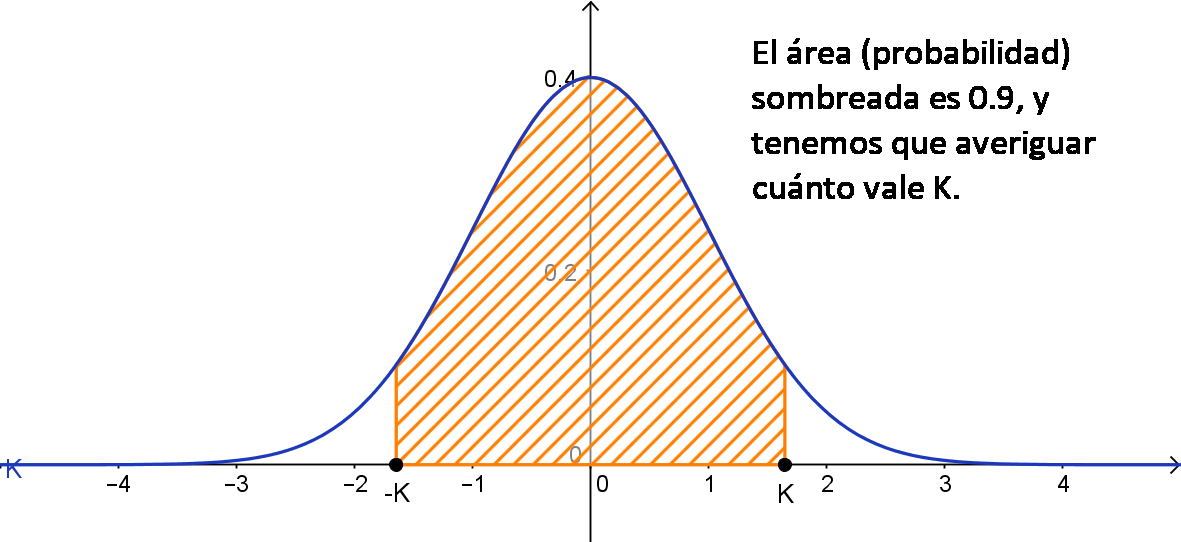
\includegraphics[width=7cm]{../fig/06-02-ProblemaInversoZ-02} \end{center}

  Sustituyendo la anterior expresión de \(Z\) aquí y despejando \(\mu\)
  obtenemos la fórmula del intervalo de confianza.
\end{itemize}

\end{frame}

\begin{frame}{Fórmula preliminar del intervalo del confianza.}
\protect\hypertarget{formula-preliminar-del-intervalo-del-confianza.}{}

\begin{itemize}
\item
  Pero antes vamos a darle un nombre a \(K\). La zona sombreada de la
  anterior figura tiene probabilidad \(nc\). Queda una probabilidad
  \[\alpha = 1 - nc\] para repartir \emph{entre las dos colas}. Así,
  \emph{cada una de las dos colas} que son iguales por simetría tiene
  una probabilidad igual a \(\dfrac{\alpha}{2}\).
\item
  Dada una probabilidad \(p\), el \textbf{valor crítico} \(z_p\) es el
  valor de la normal estándar que deja \textbf{a su derecha} esa
  probabilidad \(p\). Es decir, \(P(Z > z_p) = p\). Y por tanto,
  \(K = z_{\alpha/2}\).
\item
  Una \emph{versión preliminar} de la fórmula del intervalo de confianza
  es:

  \begin{center}
  \fcolorbox{black}{Gris025}{\begin{minipage}{10cm}
  Un intervalo de confianza $(a, b)$ al nivel $nc$ es:
  $$a = \bar X - z_{\alpha/2} \dfrac{\sigma}{\sqrt{n}}, \qquad\qquad 
  b = \bar X + z_{\alpha/2}\dfrac{\sigma}{\sqrt{n}}$$
  Que se resume así:
  $$\mu = \bar X \pm z_{\alpha/2}\dfrac{\sigma}{\sqrt{n}}$$
  \end{minipage}}
  \end{center}

  \textbf{¿Por qué preliminar?} Fíjate en que aquí aparece \(\sigma\),
  que es desconocido.
\end{itemize}

\end{frame}

\begin{frame}{La aproximación de las muestras grandes.}
\protect\hypertarget{la-aproximacion-de-las-muestras-grandes.}{}

\begin{itemize}
\item
  ¿Y si no conocemos \(\sigma\) entonces qué hacemos? Hay un remedio
  sencillo \textbf{siempre que la variable \(X\) sea normal en la
  población y además la muestra sea suficientemente grande}.
\item
  En esos casos podemos cambiar \(\sigma\) por \emph{desviación típica
  muestral} \(s\) en la primera fórmula utilizable del intervalo.

  \begin{center}
  \fcolorbox{black}{Gris025}{\begin{minipage}{10cm}
  {\bf Intervalo de confianza al nivel $nc$, población normal y muestra grande.}
  $$\mu = \bar X \,\pm\, z_{\alpha/2}\,\,\dfrac{s}{\sqrt{n}}$$
  \end{minipage}}
  \end{center}
\item
  ¿Qué es una muestra grande? \(n = 30\) puede servir, pero recomendamos
  \(n > 100\).
\item
  \textbf{Ejemplo:} una muestra de una población normal tiene estos
  \emph{valores muestrales}:
  \[n = 100,\qquad \bar X = 7.34, \qquad s = 0.31\] Sea \(nc = 0.95\)
  (luego \(\alpha = 0.05\)). Sabiendo que \(z_{\alpha/2}\approx 1.96\)
  el intervalo de confianza al 95\% que se obtiene es: \[
  \mu = \bar X \pm z_{\alpha/2}\dfrac{s}{\sqrt{n}} \approx 7.34 + 1.96 \dfrac{0.31}{\sqrt{100}} =  
  (7.279, 7.401).
  \] ¿Cómo hemos llegado a ese valor de \(z_{\alpha/2}\approx 1.96\)?
\end{itemize}

\end{frame}

\begin{frame}[fragile]{Valores críticos e intervalos de confianza con
R.}
\protect\hypertarget{valores-criticos-e-intervalos-de-confianza-con-r.}{}

\begin{itemize}
\item
  El cálculo de \(z_{\alpha/2}\) para cualquier \(\alpha\) (y cualquier
  \(nc\)) se realiza en R con \texttt{qnorm}. ¡Pero cuidado!, por
  defecto R trabaja con la cola izquierda.
\item
  Usando por ejemplo el nivel de confianza \(nc = 0.95\) calculemos el
  correspondiente valor crítico \(z_{0.025}\), que guardaremos en la
  variable \texttt{zc}:\small

\begin{Shaded}
\begin{Highlighting}[]
\NormalTok{nc =}\StringTok{ }\FloatTok{0.95}
\NormalTok{alfa =}\StringTok{ }\DecValTok{1} \OperatorTok{-}\StringTok{ }\NormalTok{nc}
\NormalTok{(}\DataTypeTok{zc =} \KeywordTok{qnorm}\NormalTok{(alfa }\OperatorTok{/}\StringTok{ }\DecValTok{2}\NormalTok{, }\DataTypeTok{lower.tail =} \OtherTok{FALSE}\NormalTok{)) }\CommentTok{# Atención, cola derecha}
\end{Highlighting}
\end{Shaded}

\begin{verbatim}
## [1] 1.959964
\end{verbatim}

  \normalsize
\item
  A partir de aquí obtener el intervalo partiendo de los valores
  muestrales es muy fácil:\small

\begin{Shaded}
\begin{Highlighting}[]
\NormalTok{n =}\StringTok{ }\DecValTok{100}
\NormalTok{barX =}\StringTok{ }\FloatTok{7.34}
\NormalTok{s =}\StringTok{ }\FloatTok{0.31}
\NormalTok{(}\DataTypeTok{intervalo =}\NormalTok{ barX }\OperatorTok{+}\StringTok{ }\KeywordTok{c}\NormalTok{(}\OperatorTok{-}\DecValTok{1}\NormalTok{, }\DecValTok{1}\NormalTok{) }\OperatorTok{*}\StringTok{ }\NormalTok{zc }\OperatorTok{*}\StringTok{ }\NormalTok{s }\OperatorTok{/}\StringTok{ }\KeywordTok{sqrt}\NormalTok{(n))}
\end{Highlighting}
\end{Shaded}

\begin{verbatim}
## [1] 7.279241 7.400759
\end{verbatim}

  \normalsize
\end{itemize}

\begin{verbatim}
## Warning: package 'MASS' was built under R version 3.5.2
\end{verbatim}

\begin{itemize}
\item
  Partiendo de un fichero csv con la muestra, como
  \link{https://raw.githubusercontent.com/fernandosansegundo/MBDFME/master/datos/06-IntervConfNormalGrande.csv}{06-IntervConfNormalGrande.csv}:\\
  \((a)\) Leemos los datos con \texttt{read.table}. \((b)\) Calculamos
  \(n\), \(\bar X\) y \(s\) con \texttt{length,\ mean,\ sd},
  respectivamente. \((c)\) Procedemos como antes.
\item
  \textbf{Ejercicio:} con los datos de ese fichero calcula un intervalo
  de confianza para la media.
\end{itemize}

\end{frame}

\begin{frame}{Cálculo del tamaño muestral necesario.}
\protect\hypertarget{calculo-del-tamano-muestral-necesario.}{}

\begin{itemize}
\item
  En la primera fórmula vimos que la \textbf{semianchura del intervalo}
  es \(\delta = z_{\alpha/2}\cdot\dfrac{\sigma_X}{\sqrt{n}}\). Esta
  cantidad es la que define la \textbf{precisión} del intervalo. Para
  conseguir una precisión \(\delta\) dada, por ejemplo \(0.0001\),
  podemos tratar de despejar en esta fórmula \(n\),el tamaño muestral
  necesario: \[ 
  z_{\alpha/2}\cdot\dfrac{\sigma}{\sqrt{n}} < \delta \qquad \Rightarrow \qquad 
  n=\left(z_{\alpha/2}\cdot\dfrac{\sigma}{\delta}\right)^2
  \] Pero de nuevo, desconocemos \(\sigma\). La solución es hacer un
  \emph{estudio piloto} con una muestra pequeña para estimar con \(s\)
  la desviación típica \(\sigma\).
\item
  \textbf{Ejemplo.} \emph{Una empresa produce unas piezas y desea
  estimar su diámetro medio (que sigue una distribución normal). Una
  muestra piloto tuvo una desviación típica \(s = 1.3\)mm. La empresa
  quiere una medida del diámetro con un error no mayor de \(0.1\)mm y un
  nivel de confianza del \(99\%.\) ¿Qué tamaño de muestra debe
  utilizarse para conseguir ese objetivo?}\\
  Se desea una precisión \(\delta=0.1\)mm. Al ser \(nc=0.99\), tenemos
  \(\frac{\alpha}{2}=0.005\), y \(z_{\alpha/2}=z_{0.1}\approx 2.58\).
  Sustituyendo \[
  n=\left(z_{\alpha/2}\cdot\dfrac{\sigma_X}{\delta}\right)^2     \approx \left(2.58\cdot\dfrac{1.3}{0.1}\right)^2\approx 1121.3
  \] Usaríamos una muestra de tamaño \(1122\) \emph{al menos} (conviene
  ser precavidos y redondear al alza).
\end{itemize}

\end{frame}

\begin{frame}[fragile]{Muestras pequeñas en poblaciones normales.}
\protect\hypertarget{muestras-pequenas-en-poblaciones-normales.}{}

\begin{itemize}
\item
  Los resultados anteriores sirven \emph{para poblaciones normales y
  muestras grandes}. ¿Qué sucede si sabemos que \textbf{la variable
  \(X\) tiene una distribución normal} en la población, pero sólo
  disponemos de una \textbf{muestra pequeña} (con \(n < 30\))?
\item
  Si la muestra es pequeña disponemos de menos información sobre la
  variable \(X\). Eso debe traducirse, necesariamente, en un intervalo
  de confianza más ancho. Student (que en realidad se llamaba
  \href{https://es.wikipedia.org/wiki/William_Sealy_Gosset}{\textcolor{blue}{William S. Gosset}})
  se dio cuenta de que en este tipo de problemas no se podía usar \(Z\)
  directamente y descubrió un sustituto, la distribución \(t\) de
  Student.
\item
  Esa distribución tiene las \emph{colas más pesadas} (con más
  probabilidad) que \(Z\). En realidad hay una \(t\) distinta para cada
  tamaño muestral. El código de este tema usa la librería
  \texttt{manipulate} de RStudio para explorar como cambia \(t\) con
  \(n\).

  \begin{center}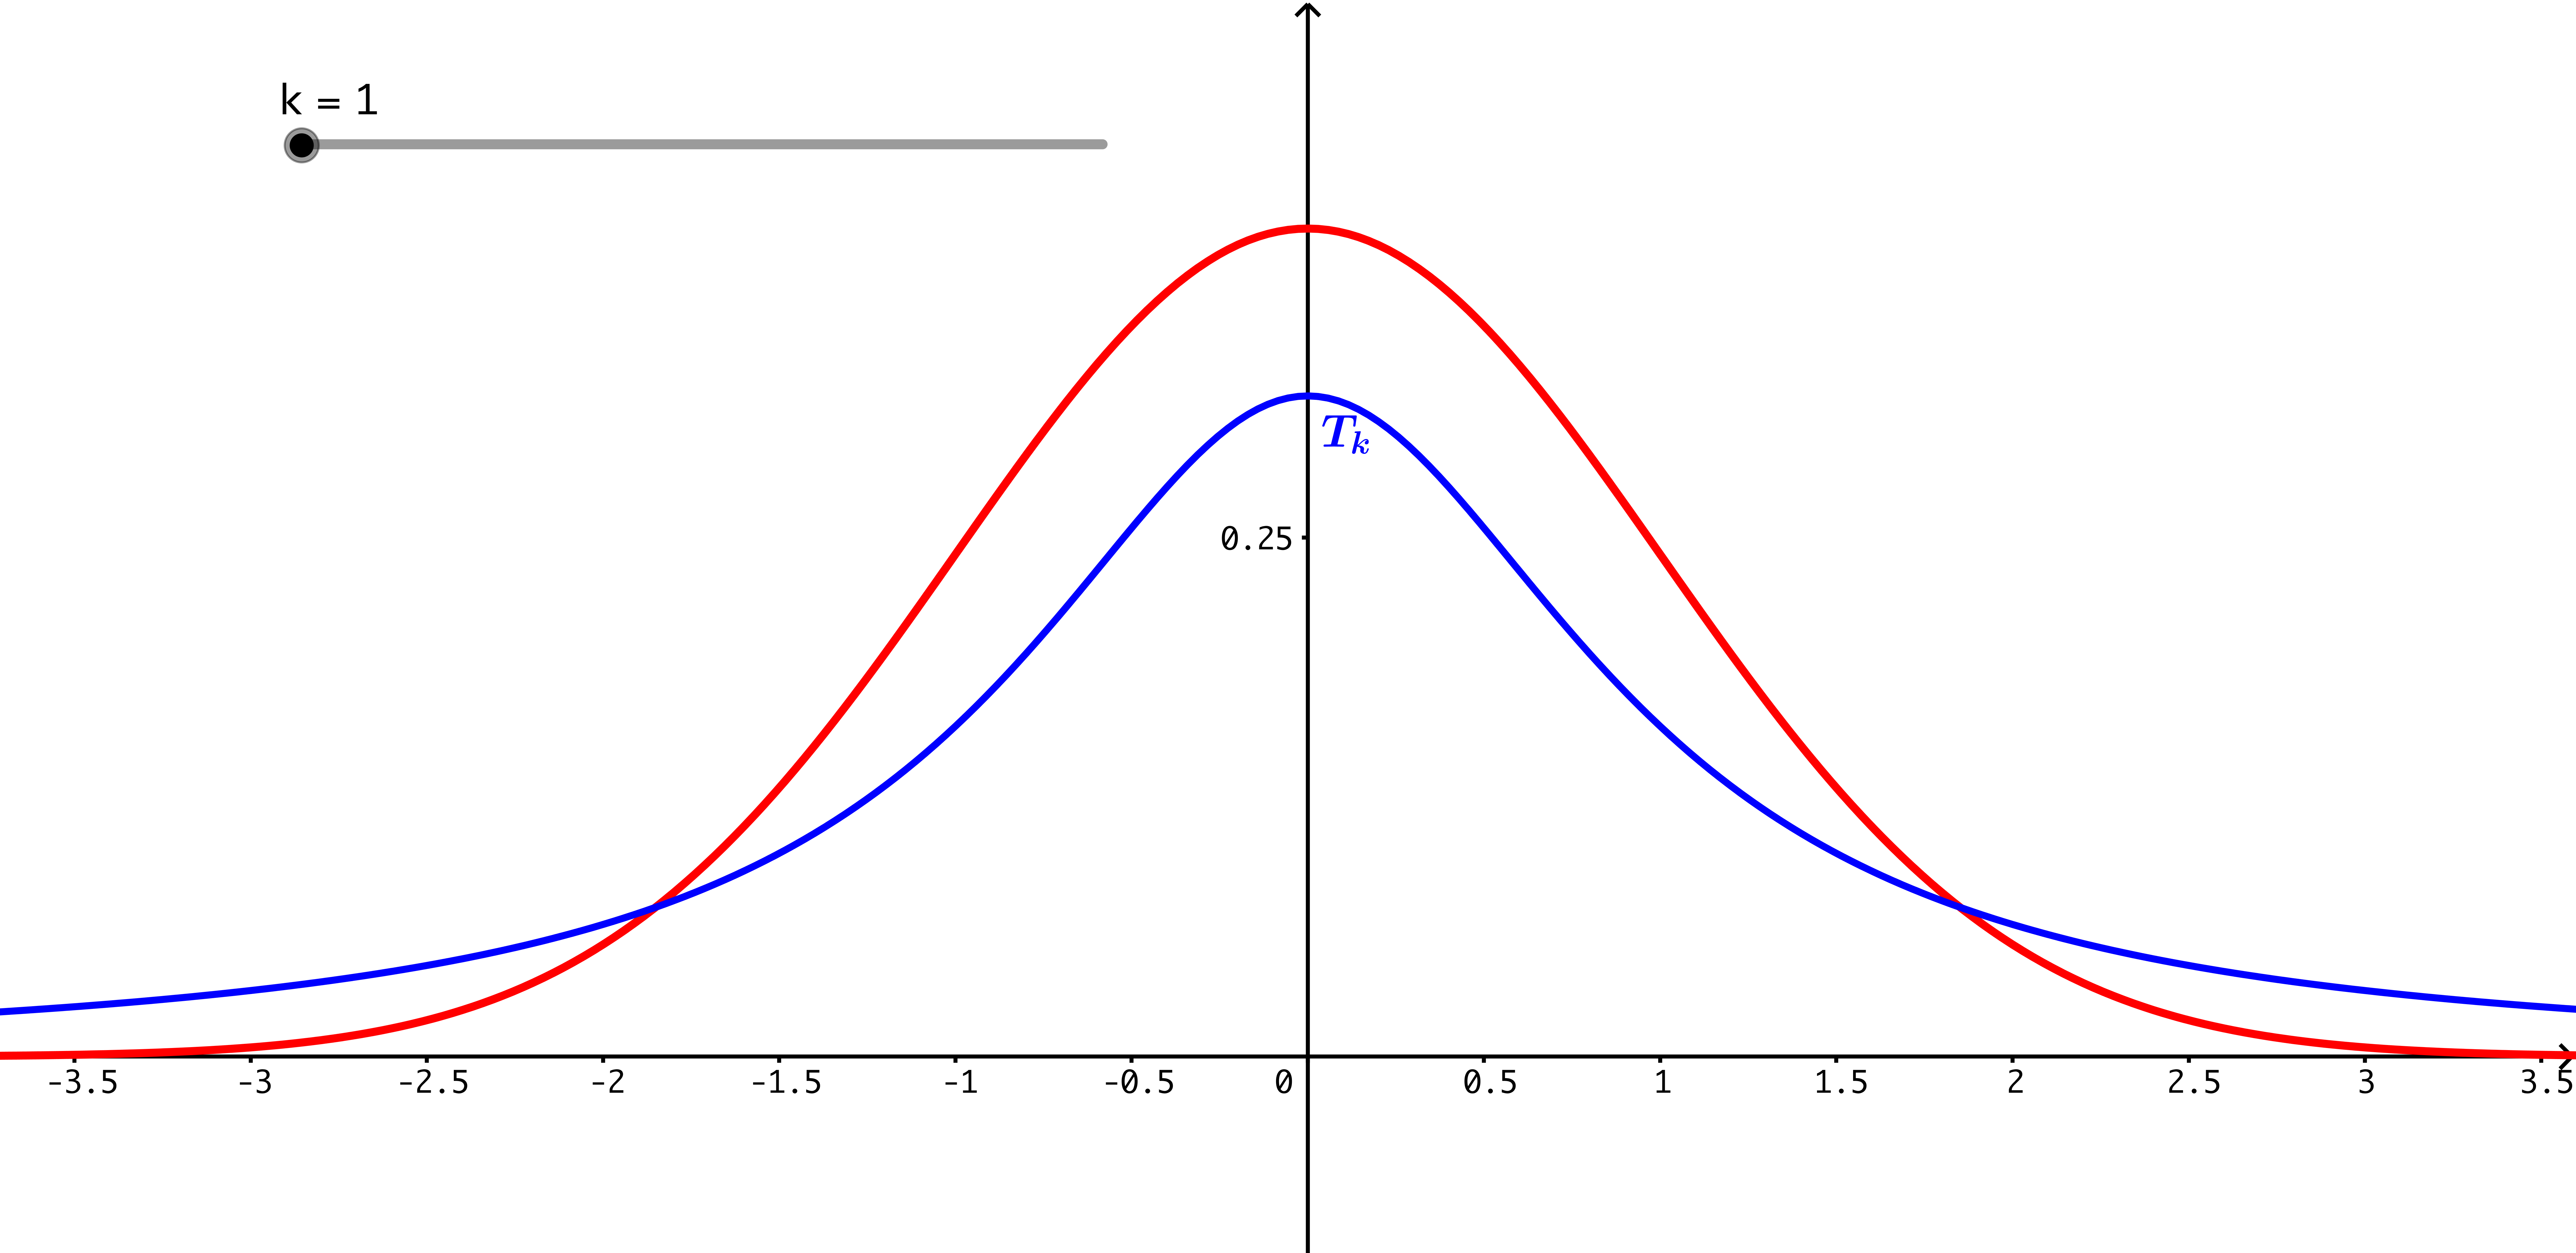
\includegraphics[width=5cm]{../fig/06-04-TvsZ} \end{center}
\end{itemize}

\end{frame}

\begin{frame}{Intervalos de confianza usando la \(t\) de Student.}
\protect\hypertarget{intervalos-de-confianza-usando-la-t-de-student.}{}

\begin{itemize}
\item
  \textbf{Grados de libertad:} Sea \(X\) una variable normal en la
  población y supongamos que el tamaño \(n\) de la muestra es pequeño.
  Diremos que \(k = n - 1\) son los grados de libertad (en inglés,
  \emph{degrees of freedom}) de esa muestra.
\item
  \textbf{Valores críticos de \(t\):}si \(T\) es una variable \(t\) de
  Student con \(k\) grados de libertad, el valor \(t_{k; p}\) verifica
  \(P(T_k > t_{k; p}) = p\) (su cola derecha tiene probabilidad \(p\)).

  \begin{center}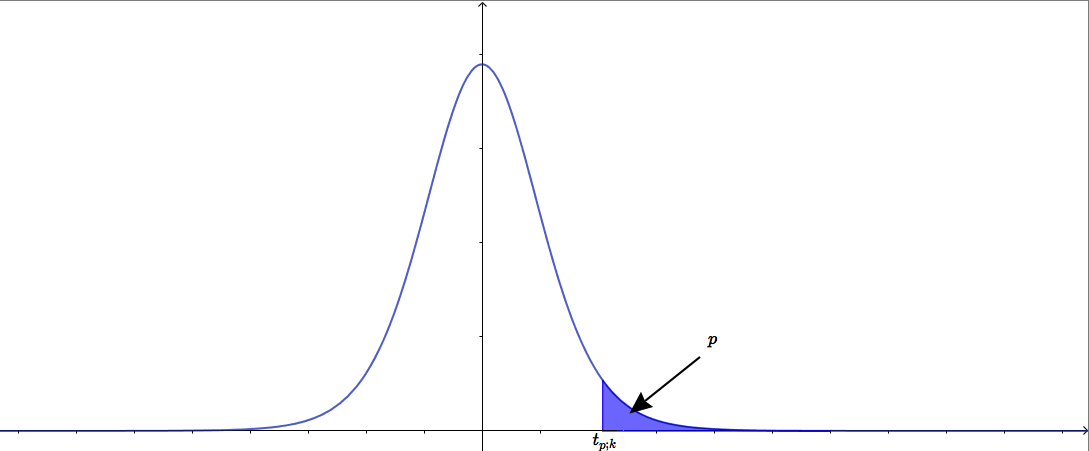
\includegraphics[width=4cm]{../fig/06-05-ValorCriticoT} \end{center}
\item
  Con esta terminología podemos dar la fórmula para el intervalo de
  confianza para \(\mu\) usando \(t\):

  \begin{center}
  \fcolorbox{black}{Gris025}{\begin{minipage}{10cm}
  {\bf Intervalo de confianza al nivel $nc$, población normal, muestra pequeña.}
  $$\mu = \bar X \pm t_{k; \alpha/2} \dfrac{s}{\sqrt{n}}$$
  \end{minipage}}
  \end{center}
\end{itemize}

\end{frame}

\begin{frame}[fragile]{La distribución \(t\) en R.}
\protect\hypertarget{la-distribucion-t-en-r.}{}

\begin{itemize}
\item
  La función \texttt{pt} es análoga a \texttt{pnorm} y sirve para el
  \emph{cálculo directo de probabilidad}. Por ejemplo, para calcular
  \(P(T_{17} > 2.5)\) (que es una cola derecha) usaríamos: \small

\begin{Shaded}
\begin{Highlighting}[]
\DecValTok{1} \OperatorTok{-}\StringTok{ }\KeywordTok{pt}\NormalTok{(}\FloatTok{2.5}\NormalTok{, }\DataTypeTok{df =} \DecValTok{17}\NormalTok{)}
\end{Highlighting}
\end{Shaded}

\begin{verbatim}
## [1] 0.0114739
\end{verbatim}

  \normalsize Fíjate en que se indican los grados de libertad con
  \texttt{df} (degrees of freedom).
\item
  \texttt{qt}, como \texttt{qnorm}, hace cálculos inversos de
  probabilidad; dada una probabilidad buscamos \emph{el valor} que deja
  esa probabilidad en su cola izquierda o derecha. Por ejemplo, para
  calcular el valor crítico \texttt{tc} para un nivel de confianza
  \texttt{nc} cualquiera haríamos:\small

\begin{Shaded}
\begin{Highlighting}[]
\NormalTok{n =}\StringTok{ }\DecValTok{20}
\NormalTok{nc =}\StringTok{ }\FloatTok{0.95}
\NormalTok{alfa =}\StringTok{ }\DecValTok{1} \OperatorTok{-}\StringTok{ }\NormalTok{nc}
\NormalTok{df =}\StringTok{ }\NormalTok{n }\OperatorTok{-}\StringTok{ }\DecValTok{1}
\NormalTok{(}\DataTypeTok{tc =} \KeywordTok{qt}\NormalTok{(alfa }\OperatorTok{/}\StringTok{ }\DecValTok{2}\NormalTok{, df, }\DataTypeTok{lower.tail =} \OtherTok{FALSE}\NormalTok{)) }\CommentTok{# Atención, cola derecha}
\end{Highlighting}
\end{Shaded}

\begin{verbatim}
## [1] 2.093024
\end{verbatim}

  \normalsize
\item
  La función \texttt{rt} sirve para simular valores aleatorios de una
  variable \(t\) de Student. \small

\begin{Shaded}
\begin{Highlighting}[]
\KeywordTok{rt}\NormalTok{(}\DecValTok{8}\NormalTok{, }\DataTypeTok{df =} \DecValTok{19}\NormalTok{)}
\end{Highlighting}
\end{Shaded}

\begin{verbatim}
## [1]  0.4187084  0.7392641  1.2306202 -1.7145000 -0.6126917
## [6]  1.1330675 -0.7748450  0.3466095
\end{verbatim}

  \normalsize
\end{itemize}

\end{frame}

\begin{frame}[fragile]{Ejemplo de cálculo de intervalo de confianza con
la \(t\) de Student.}
\protect\hypertarget{ejemplo-de-calculo-de-intervalo-de-confianza-con-la-t-de-student.}{}

\begin{itemize}
\item
  \textbf{Ejemplo:} \emph{Se sospecha que en las aguas de un embalse las
  concentraciones de nitritos superan el umbral tolerable por los peces,
  que es de 0.03 mg NO2/l o menos. Para verificar esta sospecha se
  midieron los niveles de nitritos en diez puntos aleatorios del
  embalse, obteniendo estos valores:}\\
  \(\quad\)\\
  \texttt{0.04,\ 0.05,\ 0.03,\ 0.06,\ 0.04,\ 0.06,\ 0.07,\ 0.03,\ 0.06,\ 0.02}~\\
  \(\quad\)\\
  \emph{Calculemos un intervalo de confianza al 95\% para el nivel medio
  de nitritos en las aguas del embalse. }\scriptsize   \(\quad\)

\begin{Shaded}
\begin{Highlighting}[]
\NormalTok{datos =}\StringTok{ }\KeywordTok{c}\NormalTok{(}\FloatTok{0.04}\NormalTok{, }\FloatTok{0.05}\NormalTok{, }\FloatTok{0.03}\NormalTok{, }\FloatTok{0.06}\NormalTok{, }\FloatTok{0.04}\NormalTok{, }\FloatTok{0.06}\NormalTok{, }\FloatTok{0.07}\NormalTok{, }\FloatTok{0.03}\NormalTok{, }\FloatTok{0.06}\NormalTok{, }\FloatTok{0.02}\NormalTok{)}
\NormalTok{n =}\StringTok{ }\KeywordTok{length}\NormalTok{(datos)}
\NormalTok{barX =}\StringTok{ }\KeywordTok{mean}\NormalTok{(datos)}
\NormalTok{s =}\StringTok{ }\KeywordTok{sd}\NormalTok{(datos)}
\NormalTok{nc =}\StringTok{ }\FloatTok{0.95}
\NormalTok{alfa =}\StringTok{ }\DecValTok{1} \OperatorTok{-}\StringTok{ }\NormalTok{nc}
\NormalTok{tc =}\StringTok{ }\KeywordTok{qt}\NormalTok{(}\DecValTok{1} \OperatorTok{-}\StringTok{ }\NormalTok{alfa}\OperatorTok{/}\DecValTok{2}\NormalTok{, }\DataTypeTok{df =}\NormalTok{ n }\OperatorTok{-}\StringTok{ }\DecValTok{1}\NormalTok{)}
\NormalTok{(}\DataTypeTok{intervalo =}\NormalTok{ barX }\OperatorTok{+}\StringTok{ }\KeywordTok{c}\NormalTok{(}\OperatorTok{-}\DecValTok{1}\NormalTok{, }\DecValTok{1}\NormalTok{) }\OperatorTok{*}\StringTok{ }\NormalTok{tc }\OperatorTok{*}\StringTok{ }\NormalTok{s }\OperatorTok{/}\StringTok{ }\KeywordTok{sqrt}\NormalTok{(n))}
\end{Highlighting}
\end{Shaded}

\begin{verbatim}
## [1] 0.03422133 0.05777867
\end{verbatim}

  \normalsize

  ¿Cuál es la conclusión?
\end{itemize}

\end{frame}

\begin{frame}{Resumen de intervalos de confianza para la media \(\mu\).}
\protect\hypertarget{resumen-de-intervalos-de-confianza-para-la-media-mu.}{}

\begin{itemize}
\item
  \textbf{Variable \(X\) normal y muestra grande (\(n > 100\))}:\\
  \[\mu = \bar X \pm z_{\alpha/2} \dfrac{s}{\sqrt{n}}\] En raras
  ocasiones usaremos aquí \(\sigma\) en lugar de \(s\).
\item
  \textbf{Variable \(X\) normal pero muestra pequeña}:\\
  \[\mu = \bar X \pm t_{\alpha/2;k} \dfrac{s}{\sqrt{n}}\] con
  \(k = n - 1\), los grados de libertad.
\item
  \textbf{Variable \(X\) \emph{aproximadamente normal} y muestra
  grande:}

  El TCL permite usar la fórmula previa con \(t\) para el intervalo de
  confianza.\\
  Enseguida discutiremos que significa ser aproximadamente normal.
\item
  \textbf{Variable posiblemente no normal:}

  En este caso los métodos que hemos visto no sirven para obtener un
  intervalo de confianza para la media.
\end{itemize}

\end{frame}

\begin{frame}{Intervalos de confianza por bootstrap.}
\protect\hypertarget{intervalos-de-confianza-por-bootstrap.}{}

\begin{itemize}
\item
  Muchos métodos de la Estadística clásica (intervalos de confianza,
  contrastes de hipótesis) asumen que las variables son al menos
  aproximadamente normales. Entre otras cosas, eso implica que los
  intervalos de confianza para la media son simétricos respecto a la
  media muestral. Pero a menudo encontramos muestras muy asimétricas,
  que no justifican la simetría del intervalo.
\item
  El aumento de la capacidad de cómputo ha propiciado el desarrollo de
  \textbf{métodos no paramétricos} para los intervalos de confianza
  basados en el \textbf{remuestreo}, como el \textbf{bootstrap}. Vamos a
  usar ese método para obtener un intervalo de confianza de los datos
  contenidos en el fichero
  \link{http://www.postdata-statistics.com/docs/skewdata.csv}{skewdata.csv}
  (basado en un ejemplo de (Crawley 2005, pág. 47)). La figura ilustra
  la asimetría de esos datos:
  \includegraphics{05-IntroduccionInferencia_files/figure-beamer/unnamed-chunk-14-1.pdf}
\end{itemize}

\end{frame}

\begin{frame}[fragile]{Esquema del método.}
\protect\hypertarget{esquema-del-metodo.}{}

\begin{itemize}
\item
  Empezamos leyendo esos datos (fíjate en que usamos directamente la
  URL):\small

\begin{Shaded}
\begin{Highlighting}[]
\NormalTok{x =}\StringTok{ }\KeywordTok{read.table}\NormalTok{(}\DataTypeTok{file =} \StringTok{"http://www.postdata-statistics.com/docs/skewdata.csv"}\NormalTok{, }
               \DataTypeTok{header =} \OtherTok{TRUE}\NormalTok{)[, }\DecValTok{1}\NormalTok{]}
\end{Highlighting}
\end{Shaded}

  \normalsize Ahora vamos a explorar los tamaños muestrales entre
  \(n = 5\) y \(n = 40\):

  \((a)\) Para cada tamaño construiremos \(10000\) remuestreos
  aleatorios con remplazamiento de esa muestra.

  \((b)\) En cada remuestreo calculamos la media obteniendo así 10000
  medias muestrales.

  \((c)\) Dibujamos el intervalo que va del primer al tercer cuartil de
  esas 10000 medias (todas de muestras de tamaño \(n\)).
\item
  El código R correspondiente a este esquema es muy sencillo y lo
  usaremos para introducir el uso de los bucles \texttt{for}. Al final
  de este tema hay una pequeña introducción a los bucles y estructuras
  de control en R.
\end{itemize}

\end{frame}

\begin{frame}{Representación gráfica de los intervalos bootstrap.}
\protect\hypertarget{representacion-grafica-de-los-intervalos-bootstrap.}{}

\begin{itemize}
\item
  En la gráfica el eje horizontal es el tamaño de la muestra y el
  vertical los valores de \(X\). La media de \(X\) se indica con una
  línea horizontal azul.
\item
  los intervalos bootstrap se muestran como segmentos verticales en
  naranja, la media en azul y en rojo representamos los intervalos
  \emph{clásicos} usando la \(t\) de Student. Fíjate en que para
  muestras grandes no hay apenas diferencia. Pero en muestras pequeñas
  el intervalo bootstrap refleja mucho mejor la asimetría de los datos.
\end{itemize}

\begin{center}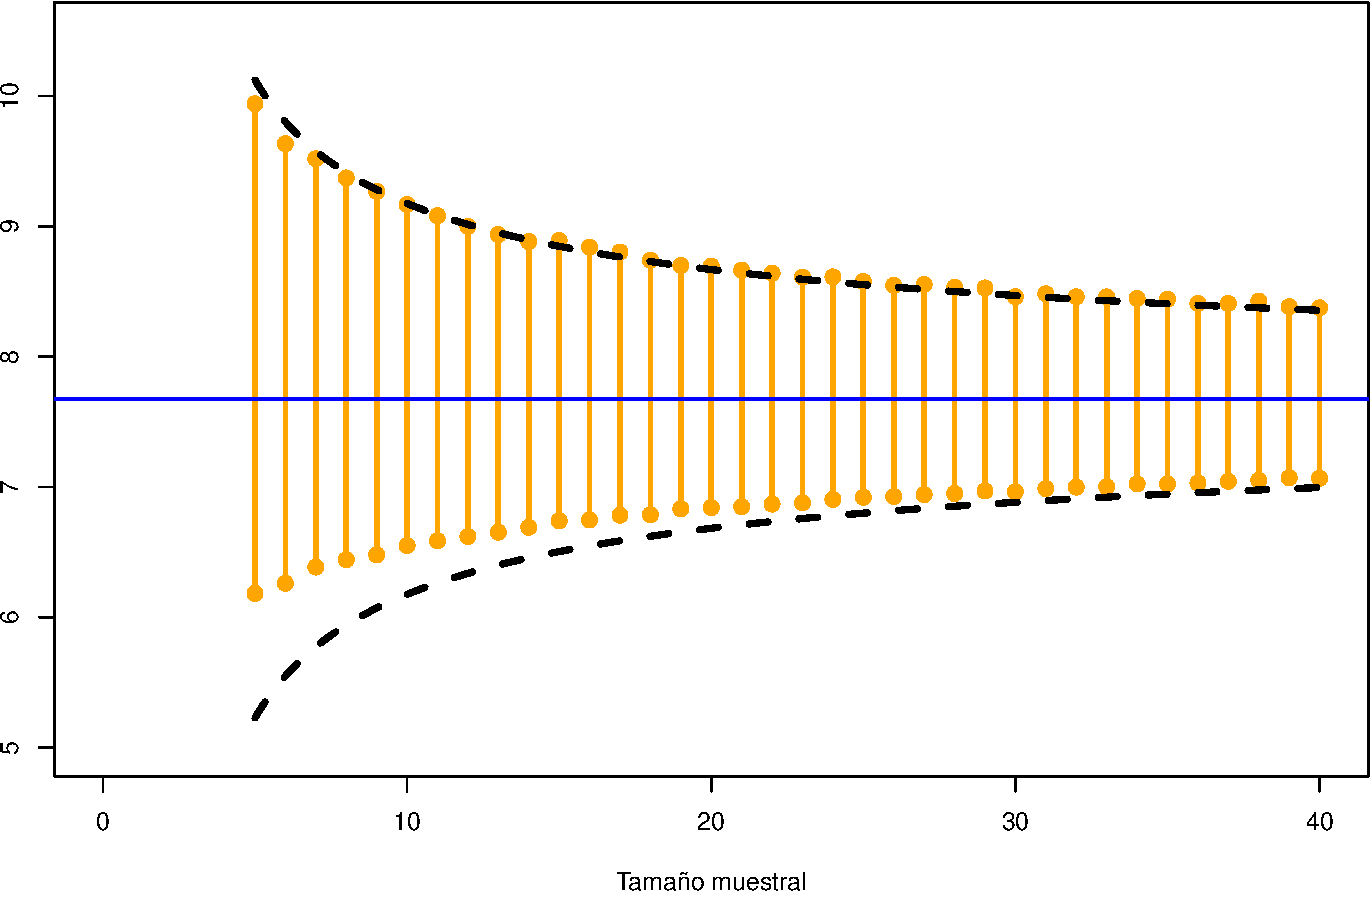
\includegraphics[width=0.6\linewidth]{05-IntroduccionInferencia_files/figure-beamer/bootstrap-1} \end{center}

\end{frame}

\begin{frame}[fragile]{Código R del bootstrap.}
\protect\hypertarget{codigo-r-del-bootstrap.}{}

\small

\begin{Shaded}
\begin{Highlighting}[]
\CommentTok{# Creamos la "caja" del gráfico.}
\KeywordTok{plot}\NormalTok{(}\KeywordTok{c}\NormalTok{(}\DecValTok{0}\NormalTok{, }\DecValTok{40}\NormalTok{), }\KeywordTok{c}\NormalTok{(}\DecValTok{5}\NormalTok{,}\FloatTok{10.5}\NormalTok{), }\DataTypeTok{type=}\StringTok{"n"}\NormalTok{, }\DataTypeTok{xlab=}\StringTok{"Tamaño muestral"}\NormalTok{, }\DataTypeTok{ylab=}\StringTok{""}\NormalTok{) }

\ControlFlowTok{for}\NormalTok{ (k }\ControlFlowTok{in} \KeywordTok{seq}\NormalTok{(}\DecValTok{5}\NormalTok{, }\DecValTok{40}\NormalTok{, }\DecValTok{1}\NormalTok{))\{ }\CommentTok{# Este bucle recorre los tamaños muestrales}
\NormalTok{  a =}\StringTok{  }\KeywordTok{numeric}\NormalTok{(}\DecValTok{10000}\NormalTok{) }\CommentTok{# el vector a almacenará las medias muestrales}
  \ControlFlowTok{for}\NormalTok{ (i }\ControlFlowTok{in} \DecValTok{1}\OperatorTok{:}\DecValTok{10000}\NormalTok{)\{ }\CommentTok{# este es el bucle de remuestreo (bootstrap)}
  \CommentTok{# generamos un remuestreo con reemp. y calculamos su media}
\NormalTok{    a[i] =}\StringTok{ }\KeywordTok{mean}\NormalTok{(}\KeywordTok{sample}\NormalTok{(x, k, }\DataTypeTok{replace=}\NormalTok{T)) }
\NormalTok{    \}}
  \CommentTok{# dibujo del intervalo bootstrap de este tamaño muestral  }
  \KeywordTok{points}\NormalTok{(}\KeywordTok{c}\NormalTok{(k,k), }\KeywordTok{quantile}\NormalTok{(a, }\KeywordTok{c}\NormalTok{(.}\DecValTok{025}\NormalTok{,.}\DecValTok{975}\NormalTok{)), }\DataTypeTok{type=}\StringTok{"o"}\NormalTok{, }
         \DataTypeTok{col =} \StringTok{"orange"}\NormalTok{, }\DataTypeTok{lwd=} \DecValTok{3}\NormalTok{) }
\NormalTok{\}}

\CommentTok{# el siguiente bloque de código genera una banda con }
\CommentTok{# los intervalos clásicos correspondientes a esas muestras.}
\NormalTok{xv =}\StringTok{ }\KeywordTok{seq}\NormalTok{(}\DecValTok{5}\NormalTok{, }\DecValTok{40}\NormalTok{, }\FloatTok{0.1}\NormalTok{) }
\NormalTok{yv =}\StringTok{ }\KeywordTok{mean}\NormalTok{(x) }\OperatorTok{-}\StringTok{ }\KeywordTok{qt}\NormalTok{(}\FloatTok{0.975}\NormalTok{, xv) }\OperatorTok{*}\StringTok{ }\KeywordTok{sqrt}\NormalTok{(}\KeywordTok{var}\NormalTok{(x) }\OperatorTok{/}\StringTok{ }\NormalTok{xv)}
\KeywordTok{lines}\NormalTok{(xv, yv, }\DataTypeTok{lty =} \DecValTok{2}\NormalTok{, }\DataTypeTok{col =} \StringTok{"black"}\NormalTok{, }\DataTypeTok{lwd =} \DecValTok{4}\NormalTok{)}
\NormalTok{yv =}\StringTok{ }\KeywordTok{mean}\NormalTok{(x) }\OperatorTok{+}\StringTok{ }\KeywordTok{qt}\NormalTok{(.}\DecValTok{975}\NormalTok{, xv) }\OperatorTok{*}\StringTok{ }\KeywordTok{sqrt}\NormalTok{(}\KeywordTok{var}\NormalTok{(x) }\OperatorTok{/}\StringTok{ }\NormalTok{xv)}
\KeywordTok{lines}\NormalTok{(xv, yv, }\DataTypeTok{lty =} \DecValTok{2}\NormalTok{, }\DataTypeTok{col =} \StringTok{"black"}\NormalTok{, }\DataTypeTok{lwd =} \DecValTok{4}\NormalTok{)}

\CommentTok{# añadimos una línea horizontal en la media}
\KeywordTok{abline}\NormalTok{(}\DataTypeTok{h =} \KeywordTok{mean}\NormalTok{(x), }\DataTypeTok{col=}\StringTok{"blue"}\NormalTok{, }\DataTypeTok{lwd=}\DecValTok{2}\NormalTok{) }
\end{Highlighting}
\end{Shaded}

\normalsize

\end{frame}

\hypertarget{intervalos-de-confianza-para-la-varianza.}{%
\section{Intervalos de confianza para la
varianza.}\label{intervalos-de-confianza-para-la-varianza.}}

\begin{frame}{Distribución muestral de \(s^2\) y la distribución
\(\chi^2\) (chi cuadrado).}
\protect\hypertarget{distribucion-muestral-de-s2-y-la-distribucion-chi2-chi-cuadrado.}{}

\begin{itemize}
\item
  Después de \(\mu\), lo natural es calcular intervalos de confianza
  para \(\sigma^2\).
\item
  Sea \(X\) de tipo \(N(\mu, \sigma)\). Lo idea natural es aproximar
  \(\sigma^2\) mediante \(s^2\). Para que la idea necesitamos algo como
  el TCL: información que relacione \(\sigma^2\) con la distribución de
  \(s^2\) en el conjunto de todas las \(n\)-muestras posibles (espacio
  muestral).
\item
  Importante: la media es una medida central y por eso era interesante
  analizar la \textbf{diferencia} \(\mu - bar X\). Pero la varianza es
  una medida de dispersión y por eso los \textbf{cocientes} son más
  útiles que las diferencias.
\item
  El resultado que necesitamos es este:

  \begin{center}
  \fcolorbox{black}{Gris025}{\begin{minipage}{10cm}
  {\bf Distribución muestral de $\sigma^2$ en poblaciones normales.}\\
  Si $X$ es una variable aleatoria de tipo $N(\mu; \sigma)$, y se utilizan muestras aleatorias
  de tamaño n, entonces:
  $$(n - 1)\dfrac{s^2}{\sigma^2} \sim \chi^2_{n - 1}$$
  siendo $\chi^2_{n - 1}$ la {\bf distribución chi cuadrado con $n-1$ grados de libertad,}
  \end{minipage}}
  \end{center}

  Veamos como es esa distribución \(\chi^2_{n - 1}\).
\end{itemize}

\end{frame}

\begin{frame}[fragile]{La distribución \(\chi^2_k\) y funciones de R.}
\protect\hypertarget{la-distribucion-chi2_k-y-funciones-de-r.}{}

\begin{itemize}
\item
  Esta distribución \emph{sólo toma valores positivos} y además es
  \emph{asimétrica}, a diferencia de la \(Z\) o la \(t\) de Student. Por
  ejemplo, la distribución \(\chi^2_4\) tiene este aspecto:

  \begin{center}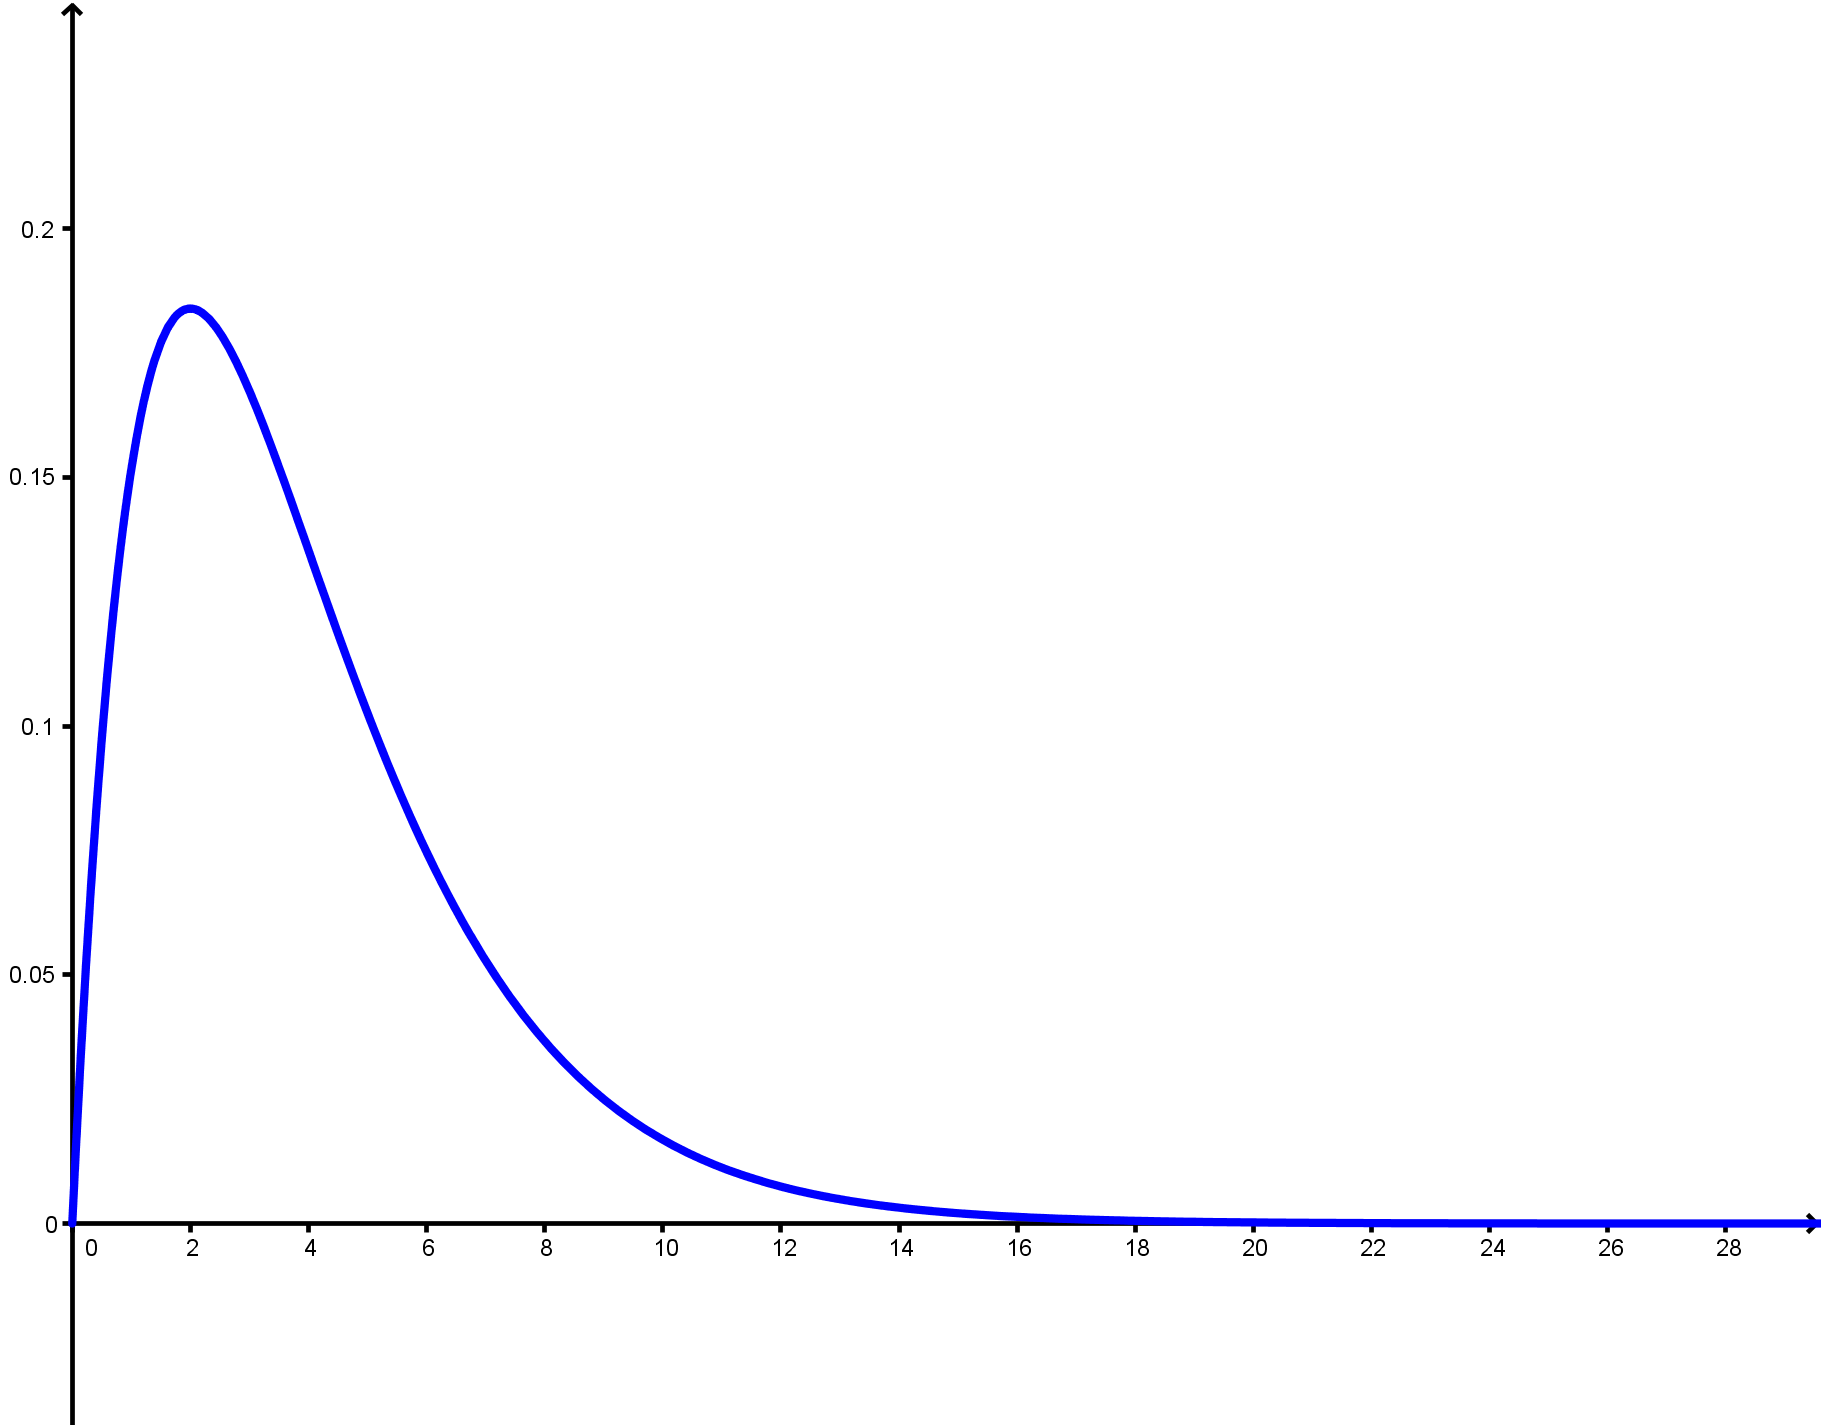
\includegraphics[width=0.5\linewidth]{../fig/06-06-DensidadChiCuadrado} \end{center}

  La asimetría, como veremos, afecta al proceso de construcción de
  intervalos de confianza basados en esta distribución.
\item
  En R disponemos de las funciones \texttt{pchisq}, \texttt{qchisq} y
  \texttt{rchisq} con los significados previsibles. El código de este
  tema usa \texttt{manipulate} para explorar esta distribución.
\end{itemize}

\end{frame}

\begin{frame}{Intervalos de confianza para la varianza.}
\protect\hypertarget{intervalos-de-confianza-para-la-varianza.-1}{}

\begin{itemize}
\item
  La novedad en este caso es que por la asimetría de \(\chi^2_k\) hay
  que usar valores críticos distintos a derecha e izquierda. Cada uno de
  ellos deja una probabilidad \(\alpha/2\) en la cola correspondiente.

  \begin{center}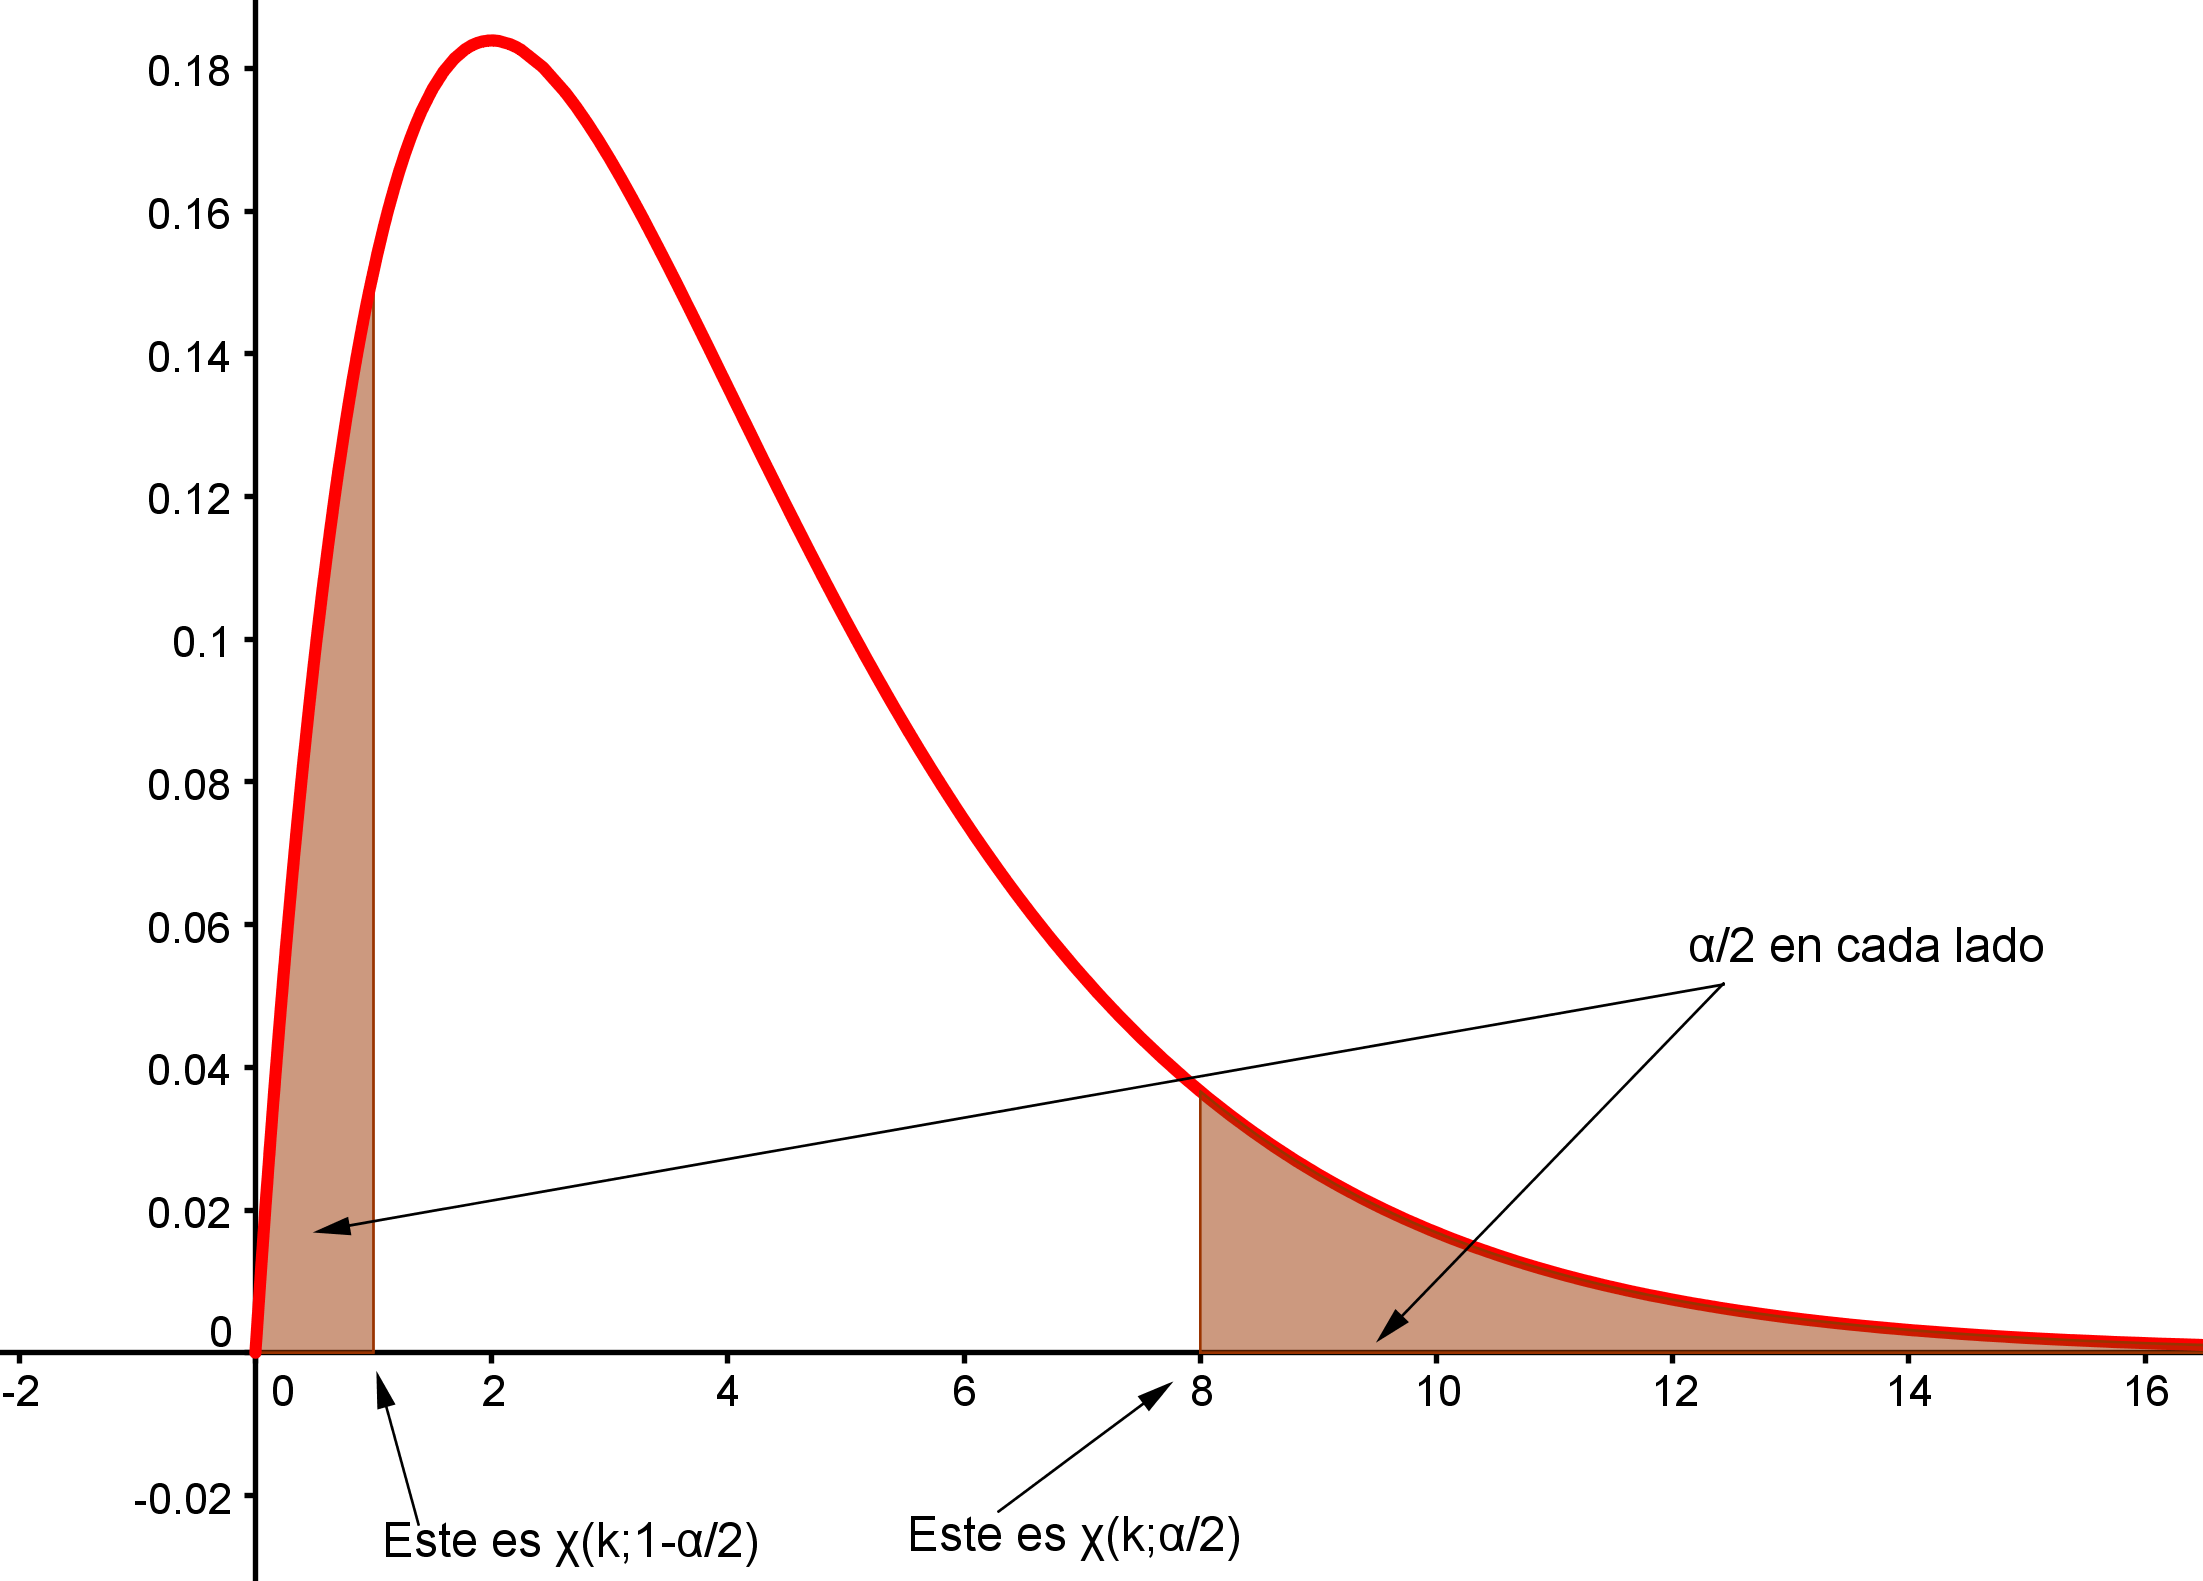
\includegraphics[width=0.45\linewidth]{../fig/06-07-ChiCuadradoValoresCriticosIntervalo} \end{center}

  donde si \(Y = \chi^2_k\) se cumple \(P(Y > \chi^2_{k, p}) = p\).

  \begin{center}
  \fcolorbox{black}{Gris025}{\begin{minipage}{10cm}
  {\bf Intervalo de confianza para  $\sigma^2$ en poblaciones normales.}\\
  $$
  \dfrac{(n-1)s^2}{\chi^2_{k,\alpha/2}}\leq\sigma^2\leq\dfrac{(n-1)s^2}{\chi^2_{k,1-\alpha/2}} ,\qquad\mbox{ con }k=n-1
  $$
  \end{minipage}}
  \end{center}
\end{itemize}

\end{frame}

\begin{frame}[fragile]{Construcción con R de intervalos de confianza
para la varianza.}
\protect\hypertarget{construccion-con-r-de-intervalos-de-confianza-para-la-varianza.}{}

\begin{itemize}
\item
  \textbf{Ejemplo:} \emph{La variable aleatoria \(X\) tiene una
  distribución normal. Una muestra aleatoria de 7 valores de \(X\) dio
  como resultado \(s^2 = 62\). Vamos a construir con R un intervalo de
  confianza (nc = 95\%) para \(\sigma^2\)}.\scriptsize

\begin{Shaded}
\begin{Highlighting}[]
\CommentTok{# Estos son los valores muestrales y el nc deseado}
\NormalTok{varianza =}\StringTok{ }\DecValTok{62} \CommentTok{# cuidado si el dato muestral es s y no s^2}
\NormalTok{n =}\StringTok{ }\DecValTok{7}
\NormalTok{nc =}\StringTok{ }\FloatTok{0.95}
\NormalTok{(}\DataTypeTok{alfa =} \DecValTok{1} \OperatorTok{-}\StringTok{ }\NormalTok{nc)}
\end{Highlighting}
\end{Shaded}

\begin{verbatim}
## [1] 0.05
\end{verbatim}

\begin{Shaded}
\begin{Highlighting}[]
\CommentTok{# Calculamos dos valores críticos de chi cuadrado.}
\NormalTok{(}\DataTypeTok{chi1 =} \KeywordTok{qchisq}\NormalTok{(alfa }\OperatorTok{/}\StringTok{ }\DecValTok{2}\NormalTok{, }\DataTypeTok{df =}\NormalTok{ n }\OperatorTok{-}\StringTok{ }\DecValTok{1}\NormalTok{, }\DataTypeTok{lower.tail =} \OtherTok{FALSE}\NormalTok{)) }\CommentTok{# cola derecha}
\end{Highlighting}
\end{Shaded}

\begin{verbatim}
## [1] 14.44938
\end{verbatim}

\begin{Shaded}
\begin{Highlighting}[]
\NormalTok{(}\DataTypeTok{chi2 =} \KeywordTok{qchisq}\NormalTok{(alfa}\OperatorTok{/}\DecValTok{2}\NormalTok{, }\DataTypeTok{df =}\NormalTok{ n }\OperatorTok{-}\StringTok{ }\DecValTok{1}\NormalTok{)) }\CommentTok{# cola izquierda}
\end{Highlighting}
\end{Shaded}

\begin{verbatim}
## [1] 1.237344
\end{verbatim}

\begin{Shaded}
\begin{Highlighting}[]
\CommentTok{# Construimos el intervalo}
\NormalTok{(}\DataTypeTok{intervalo =}\NormalTok{ (n }\OperatorTok{-}\StringTok{ }\DecValTok{1}\NormalTok{) }\OperatorTok{*}\StringTok{ }\NormalTok{varianza }\OperatorTok{/}\StringTok{ }\KeywordTok{c}\NormalTok{(chi1, chi2))}
\end{Highlighting}
\end{Shaded}

\begin{verbatim}
## [1]  25.74506 300.64390
\end{verbatim}

  \normalsize Fíjate en que el valor crítico de cola derecha se usa en
  el extremo izquierdo del intervalo y viceversa. Y si queremos un
  intervalo para \(\sigma\) simplemente calculamos la raíz cuadrada.
  \texttt{sqrt(intervalo)} produce el intervalo (5.074, 17.34) para
  \(\sigma\).
\end{itemize}

\end{frame}

\hypertarget{evaluacion-de-la-normalidad.}{%
\section{Evaluación de la
normalidad.}\label{evaluacion-de-la-normalidad.}}

\begin{frame}{¿Cómo podemos analizar la normalidad de una población?}
\protect\hypertarget{como-podemos-analizar-la-normalidad-de-una-poblacion}{}

\begin{itemize}
\item
  Los métodos de los apartados anteriores requieren evaluar si la
  variable de interés es (al menos aproximadamente) normal. En muestras
  grandes examinaremos \emph{histogramas} y \emph{curvas de densidad}.
  La figura muestra a la izquierda una muestra de datos normales y a la
  derecha datos no normales, con \(n = 500\) en ambos casos. Con
  muestras más pequeñas las cosas pueden estar menos claras.

  \begin{center}\includegraphics[width=0.65\linewidth]{05-IntroduccionInferencia_files/figure-beamer/unnamed-chunk-21-1} \end{center}

  En esta y en las siguientes páginas, mira el código de este tema.
\end{itemize}

\end{frame}

\begin{frame}{Boxplots para analizar la simetría.}
\protect\hypertarget{boxplots-para-analizar-la-simetria.}{}

\begin{itemize}
\tightlist
\item
  A menudo la simetría es el requisito más importante para que los
  métodos de la Estadística (basados en el TCL) funcionen. Los boxplots
  son especialmente útiles para detectar la falta de simetría (¡puede
  ser buena idea añadir los puntos de la muestra!).
\end{itemize}

\begin{center}\includegraphics[width=0.7\linewidth]{05-IntroduccionInferencia_files/figure-beamer/unnamed-chunk-22-1} \end{center}

\end{frame}

\begin{frame}{Violinplot.}
\protect\hypertarget{violinplot.}{}

\begin{itemize}
\tightlist
\item
  Este tipo de gráfico son interesantes al combinar la curva de densidad
  con el boxplot. Y de nuevo, es posible, añadir los puntos de la
  muestra:
\end{itemize}

\begin{center}\includegraphics[width=0.8\linewidth]{05-IntroduccionInferencia_files/figure-beamer/unnamed-chunk-23-1} \end{center}

\end{frame}

\begin{frame}{QQplots.}
\protect\hypertarget{qqplots.}{}

\begin{itemize}
\tightlist
\item
  El nombre proviene de \emph{``quantile vs quantile''}, porque se
  representa en el eje horizontal los percentiles de una variable normal
  exacta y en el vertical los de la muestra a examen. Son el tipo de
  gráficos más utilizado para analizar la normalidad. Si la muestra
  procede de una variable normal, los puntos deben coincidir con la
  recta.
\end{itemize}

\begin{center}\includegraphics[width=0.7\linewidth]{05-IntroduccionInferencia_files/figure-beamer/unnamed-chunk-24-1} \end{center}

\end{frame}

\begin{frame}{¡¡Precaución con las muestras pequeñas!!}
\protect\hypertarget{precaucion-con-las-muestras-pequenas}{}

\begin{itemize}
\tightlist
\item
  Los métodos que hemos descrito funcionan bien con muestras grandes.
  Para muestras pequeñas, las cosas se complican. Todas las figuras son
  curvas de densidad de muestras de tamaño 15 que \textbf{provienen de
  poblaciones normales}.
\end{itemize}

\begin{center}\includegraphics[width=0.85\linewidth]{05-IntroduccionInferencia_files/figure-beamer/unnamed-chunk-25-1} \end{center}

\end{frame}

\begin{frame}{Con los boxplots sucede algo parecido.}
\protect\hypertarget{con-los-boxplots-sucede-algo-parecido.}{}

\begin{itemize}
\tightlist
\item
  Todos estos boxplots son de muestras normales con \(n = 15\).
\end{itemize}

\begin{center}\includegraphics[width=11cm]{05-IntroduccionInferencia_files/figure-beamer/unnamed-chunk-26-1} \end{center}

\end{frame}

\hypertarget{contrastes-de-hipotesis.}{%
\section{Contrastes de Hipótesis.}\label{contrastes-de-hipotesis.}}

\begin{frame}{Ejemplo inicial: una discusión científica.}
\protect\hypertarget{ejemplo-inicial-una-discusion-cientifica.}{}

\begin{itemize}
\item
  Hemos desarrollado un nuevo fármaco, \emph{Pildorín Complex}, para
  tratar la depresión severa en el Canguro Rojo australiano. Pensamos
  que es tan bueno que, después de administrárselo, los pacientes darán
  saltos de alegría. De hecho, afirmamos que \emph{``la altura (media)
  de esos saltos será mayor de lo que era antes del tratamiento''.} Esta
  es nuestra \textbf{hipótesis}.
\item
  Para obtener datos relacionados con nuestra afirmación, hemos tomado
  una muestra de \(n = 100\) canguros depresivos, a los que
  administramos el medicamento. Y nos ponemos muy contentos, porque la
  altura media de sus saltos, después de usar \emph{Pildorín}, es mayor
  que antes de tratarlos.
\item
  Concretamente, un experto en canguros nos dice que la altura (en
  metros) de los saltos \textbf{se distribuye como una normal}, con
  media \[\mu_0 = 2.5\] (en metros). Pero en la muestra de 100 canguros
  depresivos tratados con \emph{Pildorín Complex} hemos observado una
  altura de salto media (muestral) \[\bar X =  2.65\] (en metros), con
  desviación típica muestral \(s = 0.5\).
\item
  Pero ese no es el final de la historia\ldots{}
\end{itemize}

\vspace{2mm}

\end{frame}

\begin{frame}{Hipótesis nula y alternativa.}
\protect\hypertarget{hipotesis-nula-y-alternativa.}{}

\vspace{4mm}

\begin{itemize}
\tightlist
\item
  El laboratorio de la competencia, que lleva años vendiendo su
  medicamento \emph{Saltaplus Forte}, dirá que nuestro medicamento tiene
  \textbf{efecto nulo} y que los saltos que hemos observado en nuestros
  canguros depresivos son, simplemente, sus saltos habituales, que los
  canguros a veces saltan más y a veces menos, y que nuestras medidas
  son simplemente \textbf{fruto del azar}. Tenemos así dos afirmaciones
  o hipótesis enfrentadas.
\end{itemize}

\vspace{2mm}

\begin{itemize}
\tightlist
\item
  La hipótesis de la competencia, que llamaremos \textbf{hipótesis nula}
  \(H_0\) (porque dice que el efecto es nulo), sostiene que la media no
  ha aumentado con el tratamiento.\vspace{2mm}\\
\item
  Nuestra hipótesis, que dice que la media sí ha aumentado. A esta la
  llamaremos \textbf{hipótesis alternativa} \(H_a\).
\end{itemize}

\vspace{2mm}

\begin{itemize}
\tightlist
\item
  Un \textbf{contraste de hipótesis} puede entenderse como la forma
  científica de resolver esta discusión, usando los datos y la teoría
  sobre Probabilidad que hemos aprendido.
\end{itemize}

\vspace{6mm}

\quad

\end{frame}

\begin{frame}{Notación.}
\protect\hypertarget{notacion.}{}

\vspace{2mm}

\begin{itemize}
\tightlist
\item
  Vamos a usar la siguiente notación, y es \textbf{muy importante}
  entenderla bien desde el principio:
\end{itemize}

\vspace{1mm}

\begin{itemize}
\tightlist
\item
  Llamaremos siempre \(\mu\) a la \textbf{media real} de la población de
  la que hemos tomado la muestra (en el ejemplo, los canguros tratados).
  Ni los defensores de \(H_0\) ni los de \(H_a\) conocen (ni es posible
  que conozcan) este valor.
\end{itemize}

\vspace{1mm}

\begin{itemize}
\tightlist
\item
  Además en la discusión ha aparecido un \textbf{valor de referencia}
  \(\mu_0 = 2.5\), que compararemos con \(\mu\) mediante muestras. Este
  valor se utiliza para formular claramente las dos hipótesis
  contrapuestas.
\end{itemize}

\vspace{1mm}

\begin{itemize}
\tightlist
\item
  Los dos valores \(\mu\) y \(\mu_0\) son \emph{valores teóricos}, no
  observados. Por último, tenemos el valor de la media muestral,
  \(\bar X\), que es un \emph{valor empírico} y procede de las
  observaciones. Pero es el valor fundamental para decidir a cuál de las
  dos hipótesis damos más credibilidad.
\end{itemize}

\vspace{1mm}

\begin{itemize}
\tightlist
\item
  Además es importante entender que ambas partes aceptan el valor de
  \(\bar X\); ese valor no se discute (sería otra discusión). Recuerda
  que usamos \(\bar X\) para \textbf{estimar} \(\mu\). Así que si
  \(\bar X\) es muy grande, ¿a quién parecen darle la razón los datos?
\end{itemize}

\end{frame}

\begin{frame}{Formalizando el contraste.}
\protect\hypertarget{formalizando-el-contraste.}{}

\begin{itemize}
\item
  La utilidad de la notación es que podemos usarla para escribir las dos
  hipótesis con más precisión:

  \((a)\) La \textbf{hipótesis alternativa} \(H_a\) sostiene que la
  media de la población (recuerda, la población es \emph{tratada}) es
  mayor que el valor de referencia. \[H_a = \{\mu > \mu_0\}\]

  \((b)\) La \textbf{hipótesis nula} \(H_0\) dice justo lo contrario:
  que la media de la población (recuerda, la población es
  \emph{tratada}) es menor o igual que el valor de referencia.
  \[H_0 = \{\mu \leq \mu_0\}\] Fíjate en que ponemos el igual en \(H_0\)
  porque si la media es igual, seguirá teniendo razón en que no ha
  habido \textbf{efecto} del tratamiento. Hay autores que siempre usan
  \(=\) en la hipótesis nula y ponen \(H_0 = \{\mu = \mu_0\}\).
\item
  \textbf{En el ejemplo:} Recuerda que era \(\mu_0 = 2.5\). Por lo tanto
  la hipótesis alternativa es \[H_a = \{\mu > 2.5\}\] mientras que la
  nula es:
  \[H_0 = \{\mu > 2.5\}\qquad (\text{ o bien } H_0 = \{\mu = 2.5\})\]
  \textbf{¡Atención!} es un error incluir la media muestral
  \(\bar X= 2.65\) en las hipótesis.
\end{itemize}

\end{frame}

\begin{frame}{La idea clave.}
\protect\hypertarget{la-idea-clave.}{}

\begin{itemize}
\item
  El punto de partida es este: dado que la muestra procede de la
  población a examen, debe ser \(\bar X\approx \mu\) y, por lo tanto, si
  \(\bar X\) es mayor que \(\mu_0\), eso parece darle la razón a
  \(H_a\).
\item
  Pero recuerda que hay \emph{``muestras malas''}. Así que el partidario
  de \(H_0\) dirá ese valor de \(\bar X\) se debe a que \textbf{por
  azar} nos ha tocado una muestra mala. Naturalmente, cuanto más grande
  sea el valor de \(\bar X\), \textbf{menos probable} es que nos haya
  tocado por azar \textbf{una muestra así de mala}.
\item
  \textbf{En el ejemplo:} el partidario de \(H_0 = \{\mu \leq 2.5\}\)
  puede entonces decir que el valor \(\bar X = 2.65\) se debe al azar y
  a una muestra desafortunada. Pero si el valor muestral hubiera sido
  \(\bar X = 5\), ese argumento de que la muestra es mala pierde mucho
  peso porque \textbf{es muy poco probable que nos toque una muestra tan
  mala}.
\item
  Para hacer de esto una discusión precisa: ¿podemos calcular esa
  probabilidad? Es decir, ¿podemos calcular la probabilidad de muestras
  tan malas como esa?
\end{itemize}

\end{frame}

\begin{frame}{Teorema Central del Límite y p-valor.}
\protect\hypertarget{teorema-central-del-limite-y-p-valor.}{}

\begin{itemize}
\item
  Lo que vamos a hacer es esto: supondremos, provisionalmente, que
  \(H_0\) es cierta. De hecho, admitiremos como correcto el valor de
  \(\mu\) que más le conviene al partidario de \(H_0\) (luego volvemos
  sobre esto). Ese valor es: \[\mu = \mu_0\]
\item
  Y ahora usaremos esa suposición provisional para calcular la
  probabilidad de una muestra \emph{tan mala o peor para \(H_0\)} como
  la nuestra. La probabilidad que vamos a calcular es el
  \textbf{p-valor} del contraste de hipótesis.
\item
  Al suponer (provisionalmente) que \(\mu = \mu_0\), podemos usar el TCL
  para decir que la distribución de la media muestral es: \[
  \bar X \sim N\left(\dfrac{\mu_0}{\frac{s}{\sqrt{n}}}\right)
  \] O, lo que es lo mismo, que \[
  \dfrac{\bar X - \mu_0}{\frac{s}{\sqrt{n}}}\sim Z
  \] Y esto nos permite calcular la probabilidad que buscamos, el
  p-valor, usando la normal estándar.
\end{itemize}

\end{frame}

\begin{frame}[fragile]{Cálculo del p-valor en el ejemplo.}
\protect\hypertarget{calculo-del-p-valor-en-el-ejemplo.}{}

\begin{itemize}
\item
  Recuerda que teníamos: \[
  \mu_0 = 2.5,\qquad n = 100,\qquad \bar X = 2.65, s = 0.5 
  \] Así que el valor de \(Z\) que obtenemos es: \[
  \dfrac{\bar X - \mu_0}{\frac{s}{\sqrt{n}}} = 
  \dfrac{2.65 - 2.5}{\frac{0.5}{\sqrt{100}}} = 3
  \] Y la siguiente figura ilustra que el p-valor es la probabilidad de
  la cola derecha de 3 en Z.

  \begin{center}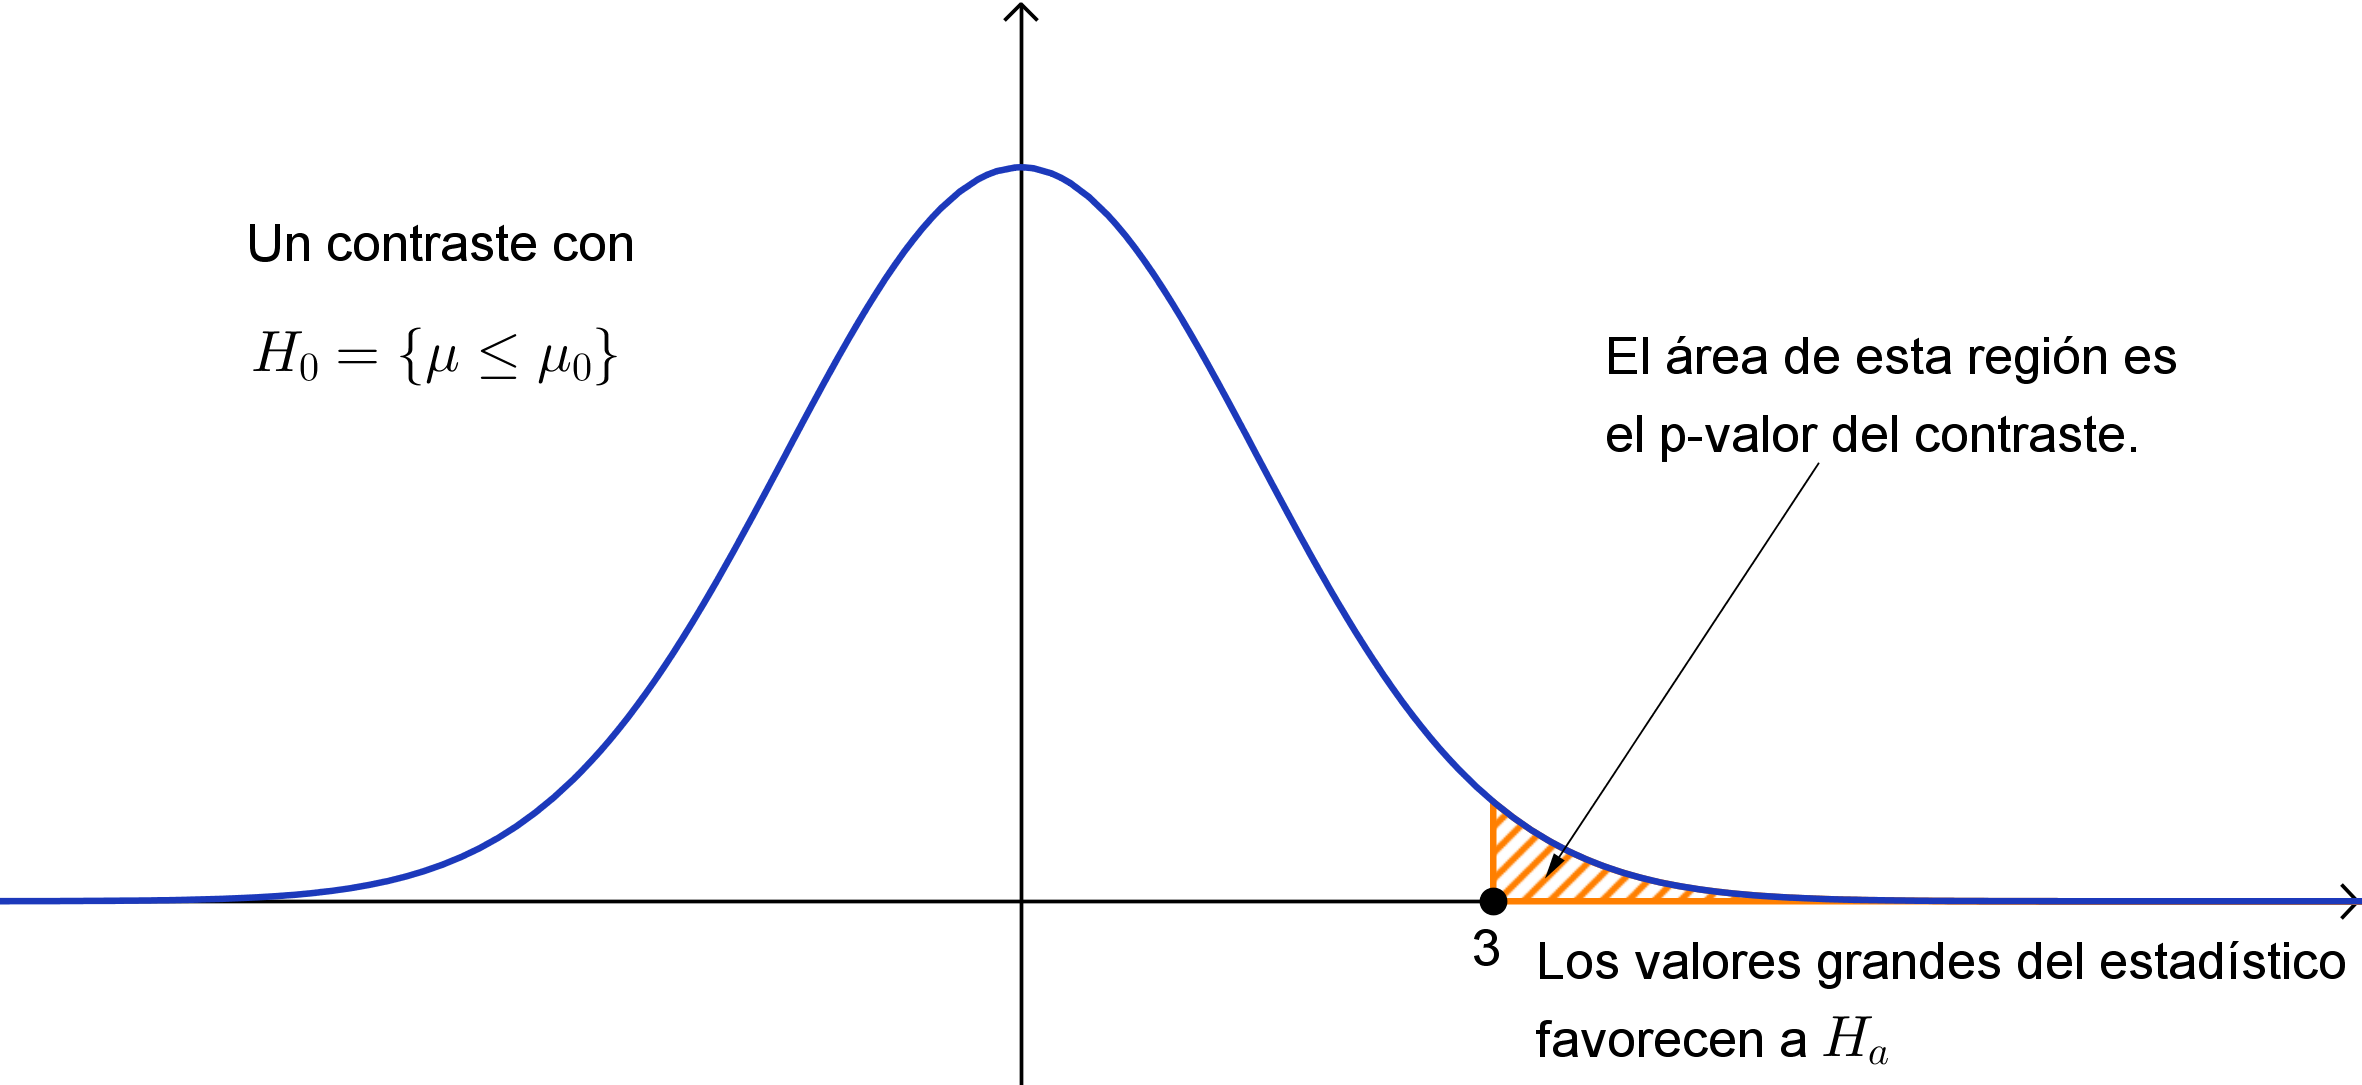
\includegraphics[width=7cm]{../fig/07-01-PValorEjemploCanguros} \end{center}
\item
  En R, obtenemos \texttt{pValor\ =\ pnorm(3,\ lower.tail\ =\ FALSE)}
  \(\approx\) 0.00135
\end{itemize}

\end{frame}

\begin{frame}[fragile]{Interpretación del resultado.}
\protect\hypertarget{interpretacion-del-resultado.}{}

\begin{itemize}
\item
  Lo que hemos hecho se puede resumir así: \emph{suponiendo que la
  hipótesis nula fuera cierta} y usando \(\mu = \mu_0\), la probabilidad
  de obtener un valor muestral tan grande o más que \(\bar X\) es de tan
  sólo 0.00135.
\item
  El partidario de \(H_0\) puede insistir en que es fruto del azar, pero
  ahora sabemos cuantificarlo. Para que el partidario de \(H_0\) tenga
  razón nos debería haber tocado una muestra tan mala que sólo hay una
  así en cada mil.
\item
  Imagínate que el valor de \(\bar X\) hubiera sido \(2.7\), más alejado
  de \(\mu_0 = 2.5\) (y por tanto más favorable a \(H_a\)). Puedes
  comprobar que el correspondiente valor de Z sería \[
  \dfrac{\bar X - \mu_0}{\frac{s}{\sqrt{n}}} = 
  \dfrac{2.7 - 2.5}{\frac{0.5}{\sqrt{100}}} = 4
  \] y entonces el p-valor habría sido aún más pequeño:
  \texttt{1\ -\ pnorm(4)} \(\approx \ensuremath{3.167\times 10^{-5}}\).
  En ese caso al partidario de \(H_0\) \emph{le costaría mucho más
  hacernos creer que todo es fruto del azar.}
\item
  En resumen, un p-valor pequeño le quita la razón al partidario de
  \(H_0\) y nos llevaría a \textbf{rechazar la hipótesis nula.}
\end{itemize}

\end{frame}

\begin{frame}{Comentarios.}
\protect\hypertarget{comentarios.}{}

\begin{itemize}
\item
  La idea del p-valor es medir \textbf{cómo de extraños, inexplicables o
  sorprendentes le parecen los resultados de la muestra a alguien que
  cree en la hipótesis nula.} Simbólicamente:
  \[\text{p-valor } = P(\text{ datos }\,|\, H_0\text{ es cierta})\]
\item
  En muchos casos la hipótesis nula representa el conocimiento
  establecido o aceptado. Y por eso, en general, debemos estar muy
  convencidos antes de rechazar la hipótesis nula. Por eso la hipótesis
  nula \emph{``juega con ventaja''.}
\item
  Por eso el valor de \(\mu = \mu_0\) es el más ventajoso para la
  hipótesis nula, Si al calcular el p-valor usáramos otro valor de
  \(\mu\) menor que \(\mu_0\) el p-valor habría sido aún más pequeño.
  Así que usamos \(\mu_0\) para darle a \(H_0\) todas las ventajas.
\item
  Y por eso incluimos todos los valores de la cola derecha. Es la misma
  idea: si tomáramos sólo una parte de esa cola la probabilidad (el
  p-valor) sería aún menor, así que usamos toda la cola.
\item
  Hemos usado el TCL para calcular el p-valor, pero también se puede
  hacer mediante remuestreo, como en el bootstrap. Esa es una opción muy
  interesante, que cada vez gana más peso en las aplicaciones. Mira el
  código de este tema.
\end{itemize}

\end{frame}

\begin{frame}[fragile]{Rechazando la hipótesis alternativa.}
\protect\hypertarget{rechazando-la-hipotesis-alternativa.}{}

\begin{itemize}
\item
  Volviendo al ejemplo que venimos usando, supongamos que hubiéramos
  obtenido \(\bar X = 2.51\), manteniendo todos los demás valores
  iguales. Entonces \[
  \dfrac{\bar X - \mu_0}{\frac{s}{\sqrt{n}}} = 
  \dfrac{2.51 - 2.5}{\frac{0.5}{\sqrt{100}}} = 0.2
  \] y el p-valor correspondiente sería: \texttt{1\ -\ pnorm(0.2)}
  \(\approx 0.4207\).\\
  Para alguien que cree que la hipótesis nula es cierta eso significa
  que el valor de \(\bar X\) que hemos obtenido no es, en absoluto, una
  sorpresa (¡la probabilidad es el 42\%!). Así que no hay evidencia,
  usando estos datos, para rechazar \(H_0\) y, en su lugar, rechazamos
  la hipótesis alternativa \(H_a\).
\item
  Hay otra situación que a veces causa confusión al principio. Desde
  luego, si hubiésemos obtenido una media muestral como
  \(\bar X = 2.45\), que es menor que \(\mu_0 = 2.5\) \textbf{no
  necesitaríamos siquiera calcular el p-valor para rechazar \(H_a\)}.
  Recuerda que creemos que \(\mu \sim \bar X\) y, por tanto, tratar de
  convencer a alguien de que \(\mu > 2.5\) enseñándole el valor
  \(\bar X = 2.45\) es una pérdida de tiempo. Pero por supuesto puedes
  calcular el valor de \(Z\) y el p-valor, que son respectivamente: \[
  \dfrac{\bar X - \mu_0}{\frac{s}{\sqrt{n}}} = 
  \dfrac{2.45 - 2.5}{\frac{0.5}{\sqrt{100}}} = -1, 
  \qquad \text{p-valor } \approx 0.8413
  \]
\end{itemize}

\end{frame}

\begin{frame}{Regla de decisión y p-valor. Nivel de significación.}
\protect\hypertarget{regla-de-decision-y-p-valor.-nivel-de-significacion.}{}

\begin{itemize}
\item
  Recuerda siempre que:\\
  \((a)\) con un \textbf{p-valor suficientemente pequeño rechazamos la
  hipótesis nula}.\\
  \((b)\) con un \textbf{p-valor grande rechazamos la hipótesis
  alternativa}
\item
  ¿Qué es un p-valor pequeño? Para que la decisión sea más objetiva y
  simple se suele utilizar un umbral de corte predeterminado, llamado el
  \textbf{nivel de significación} \emph{ns}. Entonces, los p-valores más
  pequeños que \[\alpha = 1 - ns\] se consideran suficientemente
  pequeños. Los valores más frecuentes de \emph{ns} coinciden con los
  que usamos como nivel de confianza en los intervalos, y son \(0.90\),
  \(0.95\) y \(0.99\). ¡No los confundas, son cosas distintas! Los
  correspondientes valores de \(\alpha = 1 - ns\) son \(0.10\), \(0.05\)
  y \(0.01\).
\item
  Por lo tanto, si hacemos un contraste de hipótesis usando un nivel de
  significación del \(95\%\) y obtenemos un p-valor = 0.004, puesto que
  \(1 - ns = 0.05\), teniendo en cuenta que
  \[\text{p-valor }= 0.004 < 0.05 = \alpha = \text{1 - nc}\] diremos que
  el p-valor es suficientemente pequeño y rechazamos \(H_0\). Si
  obtuviéramos, por ejemplo, un
  \(\text{p-valor }= 0.07 > 0.05 = \alpha\) rechazaríamos \(H_a\).
\end{itemize}

\end{frame}

\begin{frame}{Errores en los contrastes.}
\protect\hypertarget{errores-en-los-contrastes.}{}

\begin{itemize}
\tightlist
\item
  Al realizar un contraste de hipótesis podemos cometer dos tipos de
  errores \textbf{por la naturaleza aleatoria del proceso de muestreo}.
\end{itemize}

\begin{table}[htbp]
    \begin{center}
    \begin{tabular}{cccc}
    \cline{3-4}
    &&\multicolumn{2}{|c|}{\bf ¿Qué hipótesis es cierta?}\\[1mm]
    \cline{3-4}
                                                  &&\multicolumn{1}{|c|}{\bf $H_a$ (alternativa) es cierta}&\multicolumn{1}{|c|}{\bf $H_0$ (nula) es cierta}\\[3mm]
    \cline{2-4}
                                    &\multicolumn{1}{|c|}{\bf Rechazar $H_0$}&\multicolumn{1}{|c|}{\bf Decisión correcta}&\multicolumn{1}{|c|}{\bf Error tipo I ($\alpha$)}\\[3mm]
    \cline{2-4}
                                    &\multicolumn{1}{|c|}{\bf Rechazar $H_a$}&\multicolumn{1}{|c|}{\bf Error tipo II ($\beta$)}&\multicolumn{1}{|c|}{\bf Decisión correcta}\\[3mm]
    \cline{2-4}
    \end{tabular}
\end{center}
\end{table}

\begin{itemize}
\item
  Esta situación recuerda a la de las pruebas diagnósticas y, de hecho,
  ese lenguaje se aplica también aquí hasta cierto punto.
\item
  En muchos casos los errores de tipo I se consideran los más
  importantes. ¿Cuál es la probabilidad de cometer un error de tipo I,
  cuando usamos un nivel de significación \(ns\) (y el correspondiente
  \(\alpha = 1 - ns\))? Sería: \[
  P(\text{ rechazar }H_0\,|\, H_0\text{ es cierta})
  \] Pero eso ocurre precisamente si la muestra que hemos usado es una
  de esas muestras malas cuyo p-valor es menor que \(\alpha\). Así que
  cuando pensamos en todas ellas vemos que \textbf{la probabilidad de
  cometer un error de tipo I usando \emph{ns} es precisamente
  \(\alpha\).}
\end{itemize}

\end{frame}

\begin{frame}{Estadístico del contraste. Región de rechazo.}
\protect\hypertarget{estadistico-del-contraste.-region-de-rechazo.}{}

\begin{itemize}
\tightlist
\item
  En el ejemplo que hemos utilizado hemos organizado el cálculo del
  p-valor y la decisión del contraste este diagrama: \[
  H_0\text{ y }H_a \longrightarrow
  \text{datos muestra }n, \bar X, s \longrightarrow
  \textbf{estadístico }Z = \dfrac{\bar X - \mu_0}{\frac{s}{\sqrt{n}}} \longrightarrow
  \] \[
  \text{ p-valor usando  }Z \longrightarrow 
  \text{¿p-valor }< \alpha = 1 - ns\text{?} \longrightarrow
  \text{rechazar } H_0 \text{ o rechazar }H_a
  \]
\item
  Al hacer esto vemos que existe un valor \(z_{\alpha}\) tal que si el
  \emph{estadístico} \(Z\) calculado en la muestra cumple
  \(Z > z_{\alpha}\), entonces rechazamos \(H_0\). Esos valores del
  estadístico forman la \textbf{región de rechazo} del contraste.
\end{itemize}

\begin{center}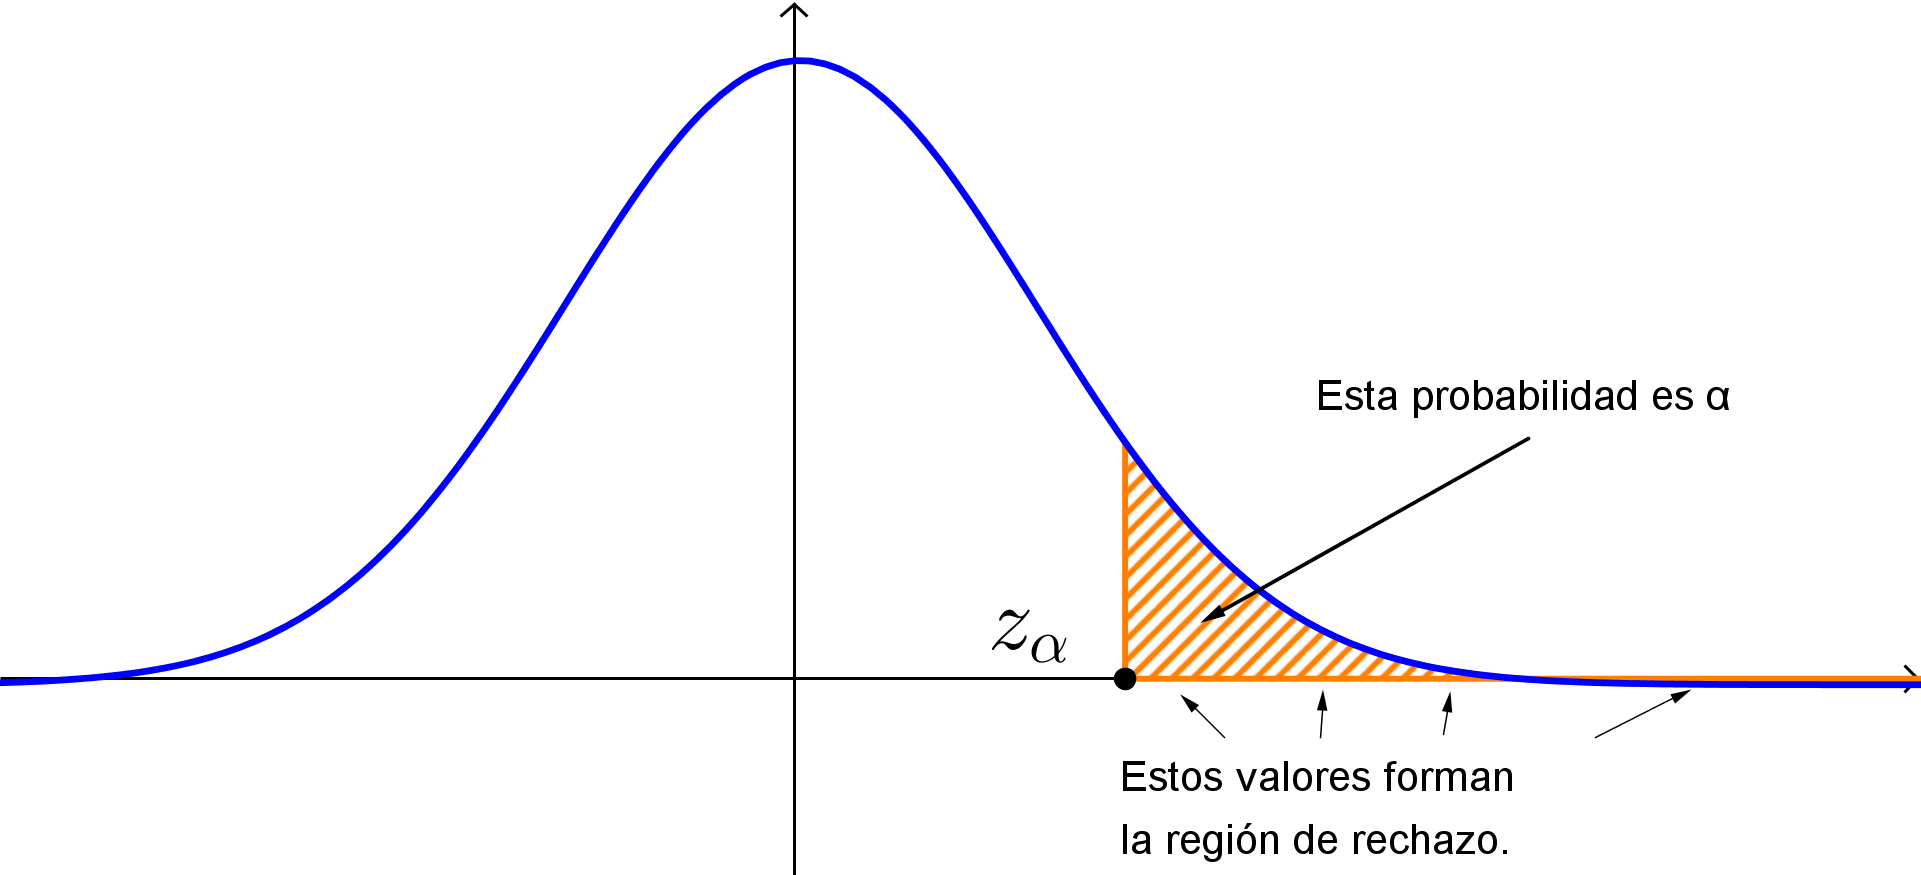
\includegraphics[width=9cm]{../fig/07-02-RegionRechazoNormalColaDerecha} \end{center}

\end{frame}

\begin{frame}{Ejemplo de región de rechazo y uso de los valores
muestrales.}
\protect\hypertarget{ejemplo-de-region-de-rechazo-y-uso-de-los-valores-muestrales.}{}

\begin{itemize}
\item
  En el caso del ejemplo que venimos usando, si queremos trabajar a un
  nivel de significación del 95\% entonces \(\alpha = 0.05\) y el valor
  \(z_{\alpha} = z_{0.05}\) es: \[
  \text{\tt qnorm(1 - 0.05)} \approx 1.645 
  \] Por lo tanto la región de rechazo la forman los valores de
  \(Z > 1.645\).
\item
  Pero también podemos expresar el valor \(Z\) a partir de los valores
  muestrales de ese ejemplo y escribir esa condición en términos de
  \(\bar X\): \[
  \dfrac{\bar X - 2.5}{\frac{0.5}{\sqrt{100}}} > 1.645
  \] Despejando de aquí el valor de \(\bar X\) obtenemos esta condición:
  \[
  \bar X >  2.582
  \] que nos indica a partir de que valores de la media muestral
  rechazaríamos \(H_0\). Pero cuidado, esto se debe interpretar con
  prudencia, porque cada muestra produce su propio valor de \(s\).
\end{itemize}

\end{frame}

\begin{frame}{Otro ejemplo de contraste de hipótesis.}
\protect\hypertarget{otro-ejemplo-de-contraste-de-hipotesis.}{}

\begin{itemize}
\item
  Vamos a pensar en otro ejemplo:\\
  \emph{La inspección de consumo está examinando un envío de latas de
  conserva, de las que el fabricante afirma que el peso medio son
  \(1000\) gramos. Al examinar una muestra aleatoria de \(100\) latas,
  un inspector obtuvo un peso medio muestral de \(998.5\) gramos, con
  una varianza muestral de \(s^2 = 36.1\) (gramos\(^2\)). Con esos
  datos, el inspector se pregunta si el peso medio de las latas será en
  realidad menor que el enunciado por el fabricante. Al nivel de
  confianza \(95\)\%, ¿qué responderías a la pregunta del inspector?
  Queremos, además, obtener el p-valor de este contraste.}
\item
  Vamos a tomar como valor de referencia \(\mu_0 = 1000\)g, como afirma
  el fabricante. Es importante entender que el peso medio real \(\mu\)
  no se conoce. La sospecha del inspector se puede traducir en forma de
  esta hipótesis alternativa:
  \[H_a:\{\mu < \mu_0\},\quad\text{ con }\mu_0 = 1000\] a la que
  corresponde la hipótesis nula: \[H_0:\,\{\mu \geq \mu_0\}\] Las
  desigualdades en estas hipótesis tienen el sentido contrario al del
  ejemplo inicial con los canguros.
\end{itemize}

\end{frame}

\begin{frame}{Cálculo del p-valor.}
\protect\hypertarget{calculo-del-p-valor.}{}

\begin{itemize}
\item
  El esquema es muy parecido al que hemos usado en el primer ejemplo,
  pero la figura de referencia ahora es esta:

  \begin{center}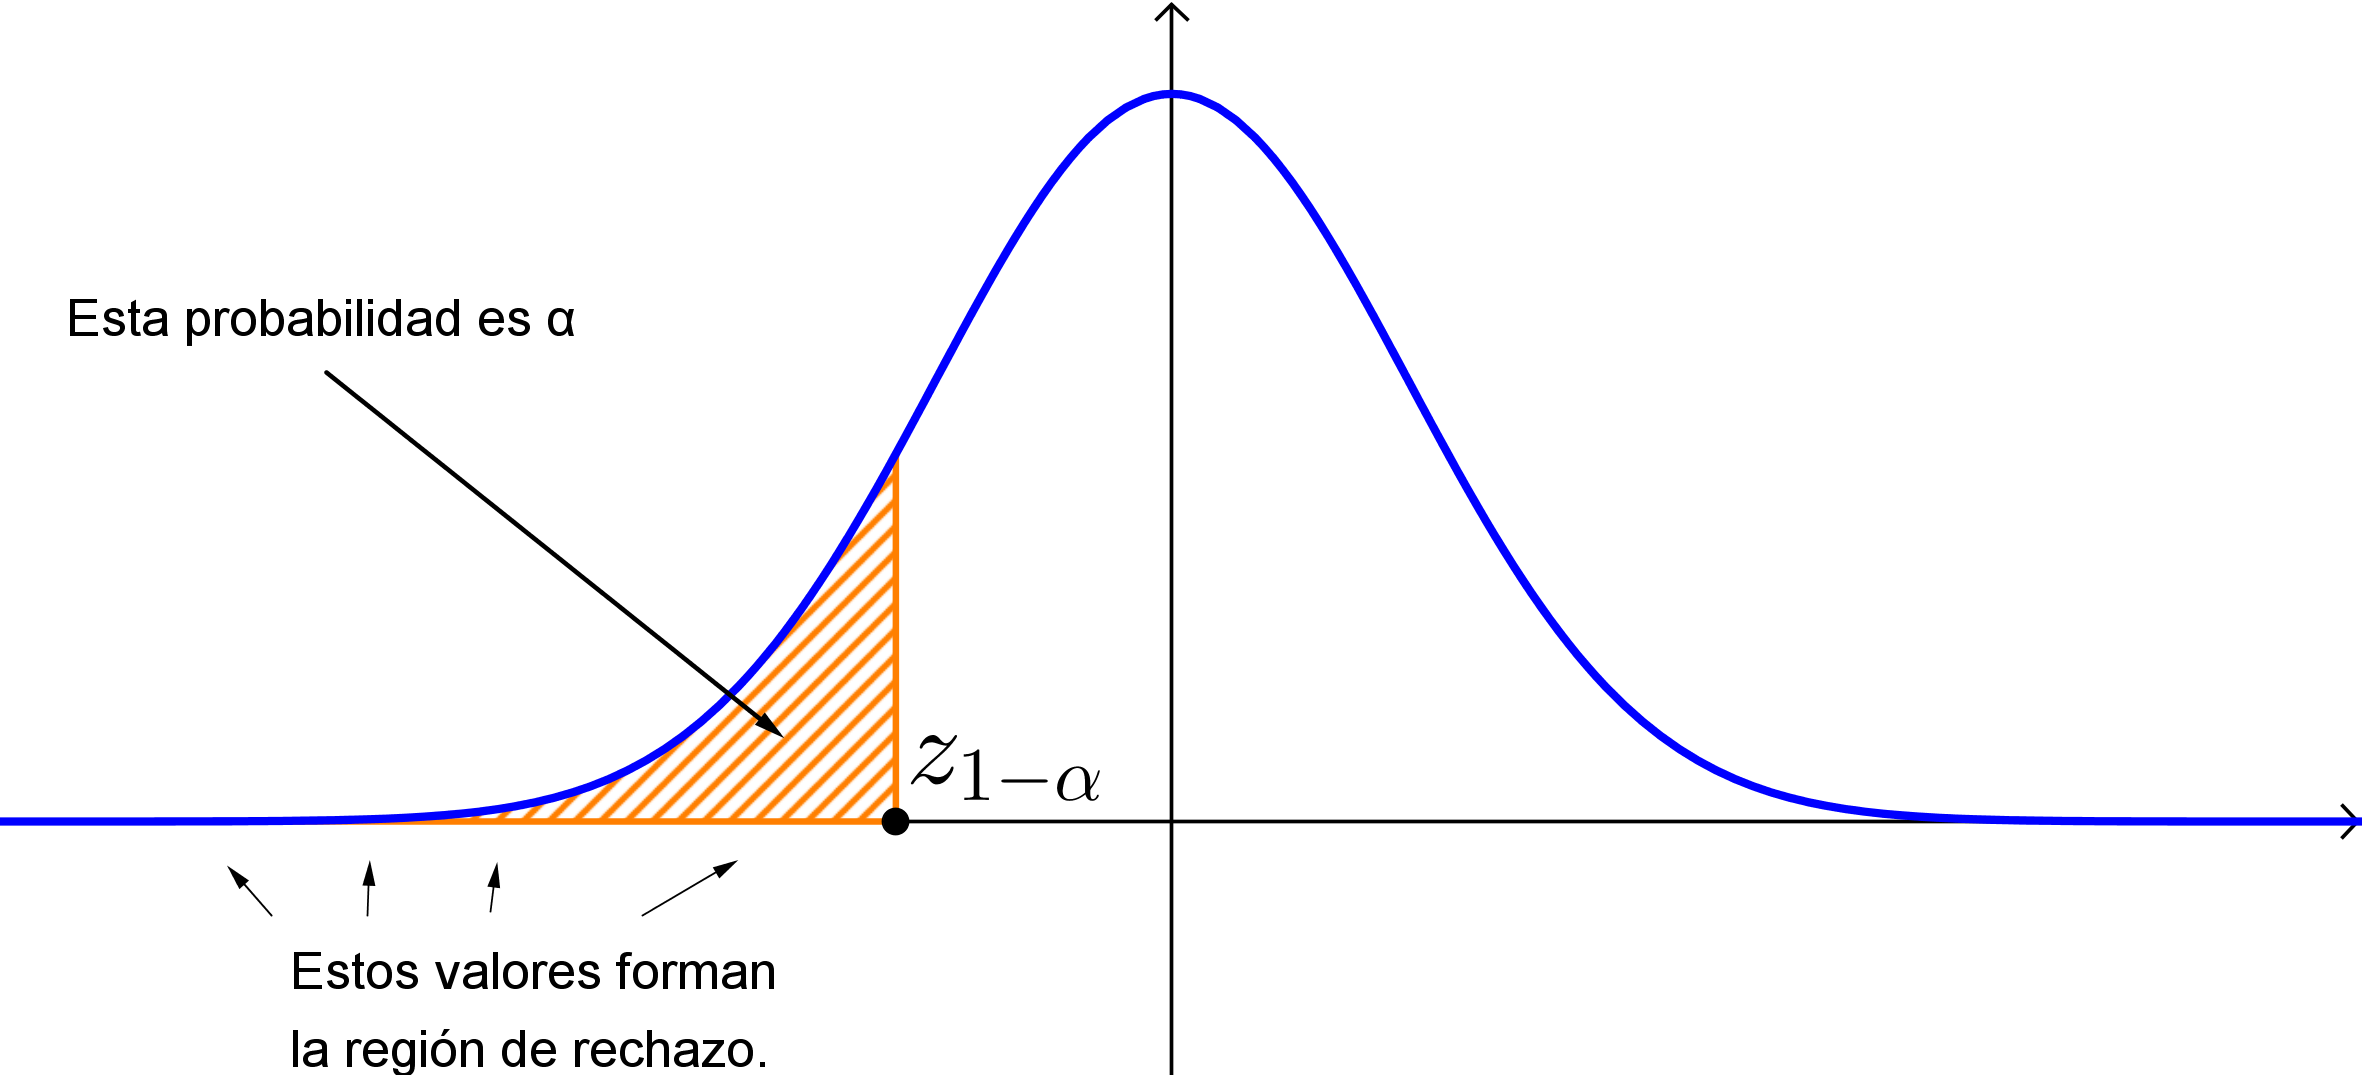
\includegraphics[width=6cm]{../fig/07-03-RegionRechazoNormalColaIzquierda} \end{center}

  Calculamos el estadístico que es, naturalmente, negativo:
  \[\dfrac{\bar X - \mu_0}{\frac{s}{\sqrt{n}}} = 
  \dfrac{998.5 - 1000}{\sqrt{\frac{36.1}{100}}} \approx 
  -2.497
  \]
\item
  El p-valor ahora es la probabilidad de la cola izquierda del
  estadístico: \[
  \text{\tt pnorm((998.5 - 1000)/sqrt(36.1/100))} \approx 0.006262
  \] Comparamos el p-valor con \(\alpha = 0.05\) y al ser p-valor
  \(< \alpha\), rechazamos \(H_0\). Con esos datos rechazamos que el
  peso medio de las latas sea \(\geq 1000g\).
\end{itemize}

\end{frame}

\begin{frame}{Contraste bilateral.}
\protect\hypertarget{contraste-bilateral.}{}

\begin{itemize}
\item
  Pensemos el mismo problema desde la perspectiva del fabricante. Al
  inspector le preocupa que el peso de las latas pueda ser menor que
  \(1000g\), porque eso podría ser un fraude a los consumidores (pero si
  el fabricante decide envasar en cada lata más producto del que
  anuncia, el inspector no pondrá pegas).
\item
  En cambio la decisión del fabricante es más complicada:

  \(-\) si envasa demasiado poco producto, el inspector le sancionará.\\
  \(-\) si, para evitar eso, envasa demasiado producto en cada lata,
  estará perdiendo dinero.
\item
  ¿Cuál debe ser entonces su objetivo? Lo razonable es intentar que la
  cantidad de producto envasado se parezca mucho al objetivo marcado
  \(\mu_0=1000\) gramos. Así que el fabricante tratará de cumplir la
  hipótesis nula (bilateral): \[ H_0=\{\mu = \mu_0\}.\] El departamento
  de control de calidad de la fábrica trabajará para contrastar esta
  hipótesis frente a la hipótesis alternativa
  \[ H_a=\{\mu\neq \mu_0\}.\]
\item
  En un contraste bilateral es más difícil rechazar \(H_0\). Por eso, si
  hay \emph{``presunción de inocencia''} para \(H_0\) se suelen usar
  contrastes bilaterales.
\end{itemize}

\end{frame}

\begin{frame}{Cálculo del p-valor en el caso bilateral. ¡¡Cuidado!!}
\protect\hypertarget{calculo-del-p-valor-en-el-caso-bilateral.-cuidado}{}

\begin{itemize}
\tightlist
\item
  En este caso al defensor de la hipótesis nula le preocupa por igual
  alejarse de \(\mu_0\) hacia valores más bajos o más altos. La figura
  que refleja esa situación es:
\end{itemize}

\begin{center}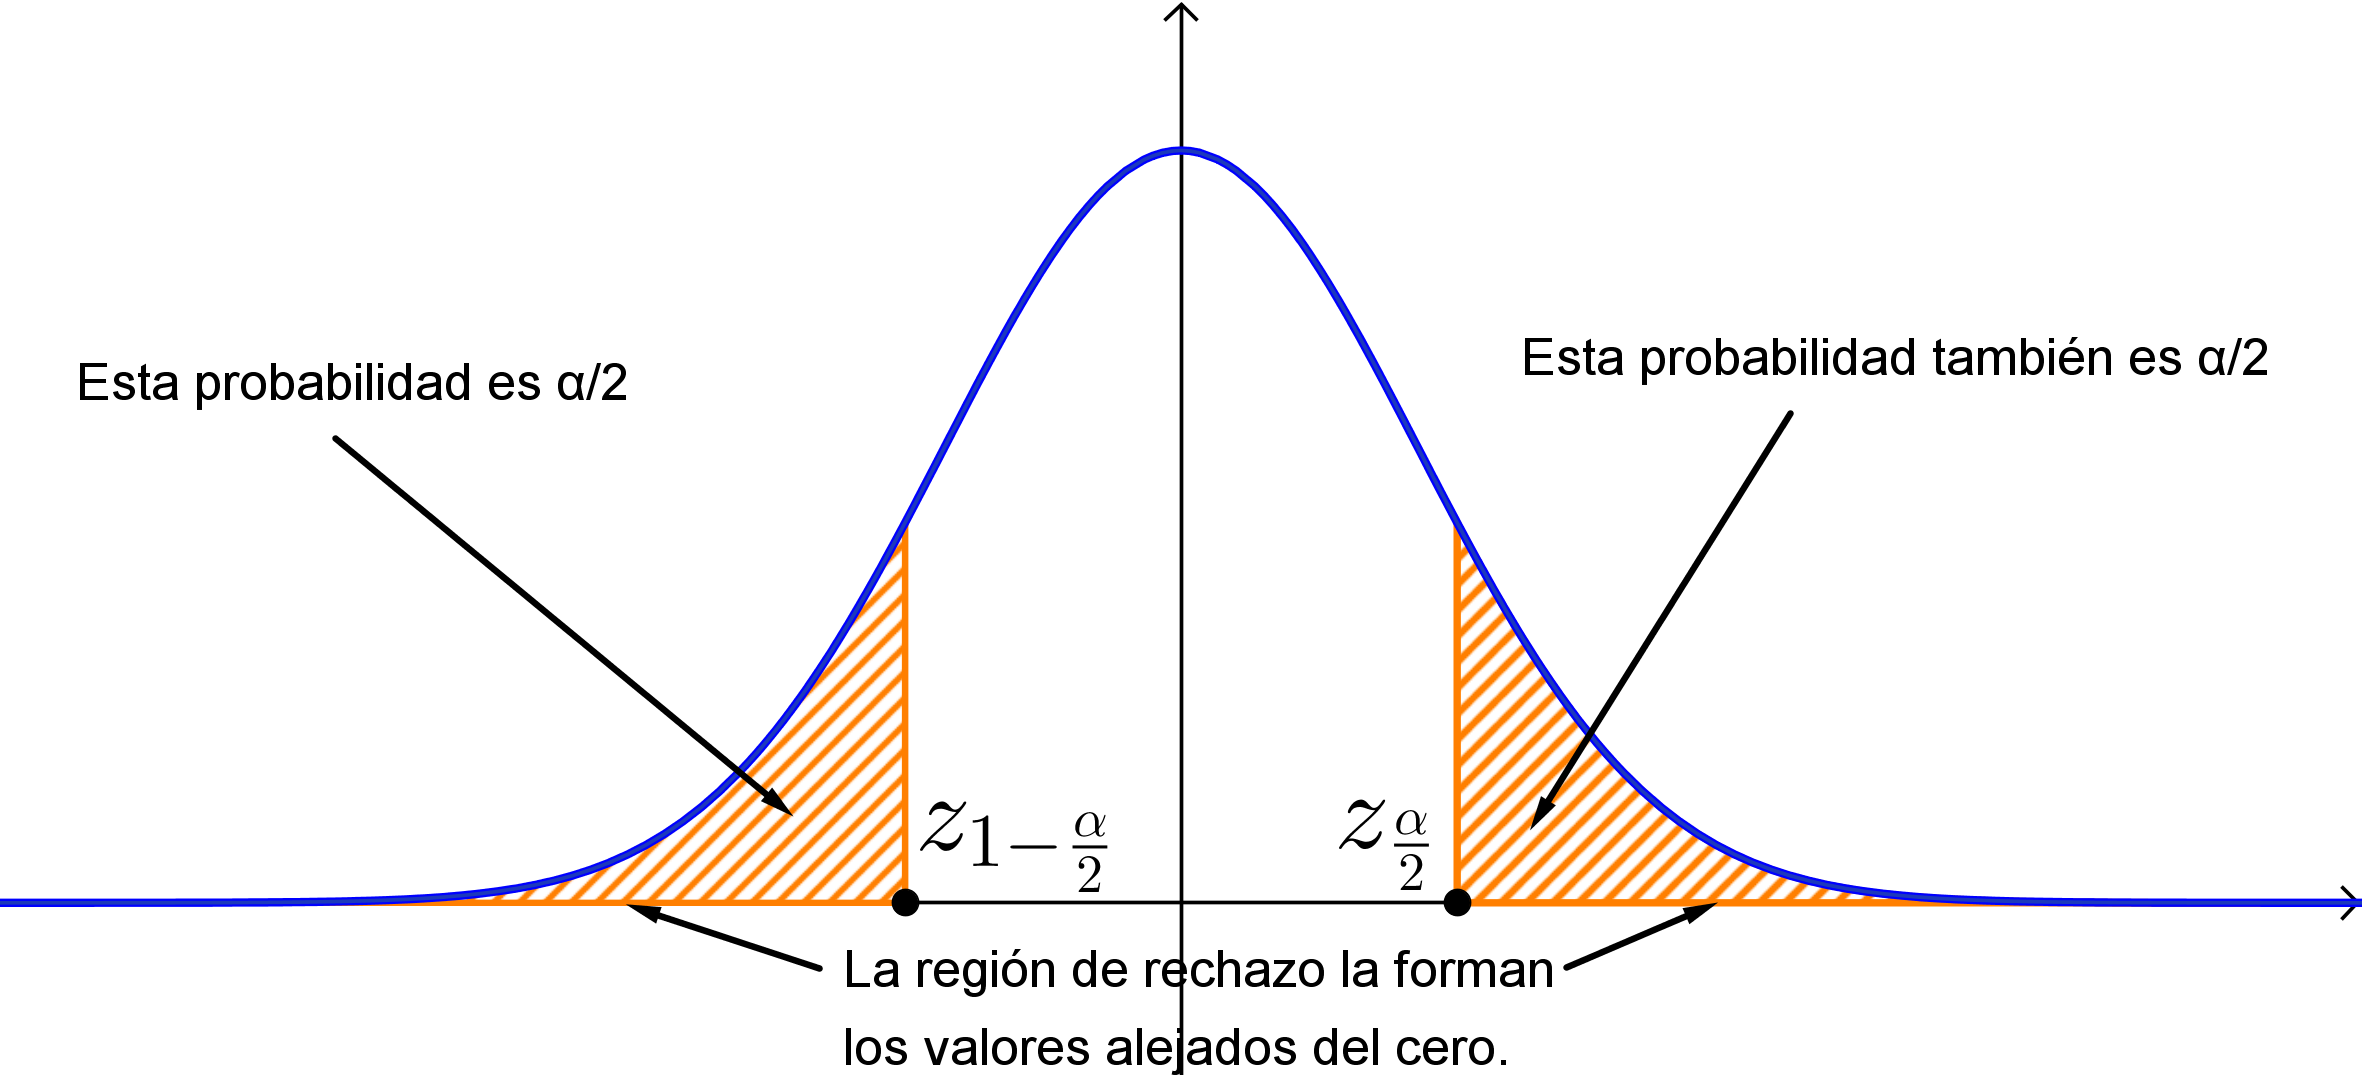
\includegraphics[width=6cm]{../fig/07-04-RegionRechazoNormalBilateral} \end{center}

Por eso, al calcular el estadístico del contraste incluimos un valor
absoluto:\small
\[\text{estadistico} = \left|\dfrac{\bar X - \mu_0}{\frac{s}{\sqrt{n}}}\right| = 
  \left|\dfrac{998.5 - 1000}{\sqrt{\frac{36.1}{100}}} \right|\approx 
  2.497
  \]\normalsize + Al calcular el p-valor \textbf{sumamos la probabilidad
de las dos colas}, multiplicando por 2: \[
  \text{\tt 2 * pnorm(estadistico, lower.tail = FALSE)} \approx 0.01252
  \] En este caso, con \(ns = 0.95\) también rechazaríamos la \(H_0\).

\end{frame}

\begin{frame}{Contrastes sobre la media con muestras pequeñas en
variables normales.}
\protect\hypertarget{contrastes-sobre-la-media-con-muestras-pequenas-en-variables-normales.}{}

\begin{itemize}
\item
  El contraste es análogo, cambiando \(Z\) por la \(t_k\), siendo \(k\)
  el tamaño de la muestra.
\item
  \textbf{Ejemplo:} Vamos a hacer el contraste:
  \[H_0 = \{\mu \geq 4\}, \qquad H_a = \{\mu < 4\}\] con \(ns = 99\%\) y
  estos datos muestrales: \[
  n = 21,\qquad \bar X = 3.6, \qquad s = 0.6
  \]
\item
  El valor de referencia es \(\mu_0 = 4\), así que el estadístico es: \[
  T = \dfrac{\bar X - \mu_0}{\frac{s}{\sqrt{n}}} =
  \dfrac{3.6 - 4}{\frac{0.6}{\sqrt{21}}}\approx
  -3.055
  \] Aunque la fórmula es la misma, lo llamamos \(T\) porque usamos la
  \(t_k\) de Student (con \(k = n - 1 = 20\)) para calcular el p-valor:
  \[
  \text{ \tt pValor = pt(estadistico, df = n - 1)} \approx 0.003125
  \] ¿Cuál es la decisión?
\item
  Los otros tipos de contrastes son similares, cambiando \(Z\) por la
  \(t_k\).
\end{itemize}

\end{frame}

\begin{frame}[fragile]{La función \texttt{t.test} de R.}
\protect\hypertarget{la-funcion-t.test-de-r.}{}

\begin{itemize}
\item
  Usar siempre \texttt{pnorm} para hacer contrastes no es cómodo ni
  eficiente. Por eso no existe \texttt{t.test}.
\item
  \textbf{Ejemplo:} Vamos a usar \texttt{t.test} con los datos de la
  variable \texttt{cty} en la tabla \texttt{mpg} (librería
  \texttt{tidyverse}) para contrastar la hipótesis alternativa:
  \[H_a =\{\mu \neq 16\}\] \small

\begin{Shaded}
\begin{Highlighting}[]
\KeywordTok{library}\NormalTok{(tidyverse)}
\NormalTok{(}\DataTypeTok{testCty =} \KeywordTok{t.test}\NormalTok{(mpg}\OperatorTok{$}\NormalTok{cty, }\DataTypeTok{mu =} \DecValTok{16}\NormalTok{, }
                  \DataTypeTok{alternative =} \StringTok{"two.sided"}\NormalTok{, }\DataTypeTok{conf.level =} \FloatTok{0.95}\NormalTok{))}
\end{Highlighting}
\end{Shaded}

\begin{verbatim}
## 
##    One Sample t-test
## 
## data:  mpg$cty
## t = 3.0874, df = 233, p-value = 0.002264
## alternative hypothesis: true mean is not equal to 16
## 95 percent confidence interval:
##  16.31083 17.40712
## sample estimates:
## mean of x 
##  16.85897
\end{verbatim}

  \normalsize Las \(H_a\) para contrastes unilaterales se indican con
  \texttt{less} y \texttt{greater}.
\end{itemize}

\end{frame}

\begin{frame}[fragile]{Detalles adicionales sobre \texttt{t.test}}
\protect\hypertarget{detalles-adicionales-sobre-t.test}{}

\begin{itemize}
\item
  Asignar el resultado de \(t.test\) a una variable permite acceder a
  componentes de la respuesta. Por ejemplo, el p-valor:\small

\begin{Shaded}
\begin{Highlighting}[]
\NormalTok{testCty}\OperatorTok{$}\NormalTok{p.value}
\end{Highlighting}
\end{Shaded}

\begin{verbatim}
## [1] 0.002263908
\end{verbatim}

  \normalsize
\item
  Además \texttt{t.test} también calcula un intervalo de confianza para
  la media:\small

\begin{Shaded}
\begin{Highlighting}[]
\NormalTok{testCty}\OperatorTok{$}\NormalTok{conf.int}
\end{Highlighting}
\end{Shaded}

\begin{verbatim}
## [1] 16.31083 17.40712
## attr(,"conf.level")
## [1] 0.95
\end{verbatim}

  \normalsize Si el contraste es unilateral R produce un intervalo de
  confianza \emph{no acotado}. Por ejemplo, si para la variable
  \texttt{displ} de \texttt{mpg} contrastamos
  \(H_a = \{\mu > 3.4\}\)\small

\begin{Shaded}
\begin{Highlighting}[]
\NormalTok{testDispl =}\StringTok{ }\KeywordTok{t.test}\NormalTok{(mpg}\OperatorTok{$}\NormalTok{displ,  }\DataTypeTok{mu =} \FloatTok{3.4}\NormalTok{, }
                    \DataTypeTok{alternative =} \StringTok{"greater"}\NormalTok{, }\DataTypeTok{conf.level =} \FloatTok{0.95}\NormalTok{)}
\NormalTok{testDispl}\OperatorTok{$}\NormalTok{conf.int}
\end{Highlighting}
\end{Shaded}

\begin{verbatim}
## [1] 3.332319      Inf
## attr(,"conf.level")
## [1] 0.95
\end{verbatim}

  \normalsize El intervalo (al 95\%) para \(\mu\) es
  \((3.332, +\infty)\)
\end{itemize}

\end{frame}

\begin{frame}{Contrastes de hipótesis para la varianza.}
\protect\hypertarget{contrastes-de-hipotesis-para-la-varianza.}{}

\begin{itemize}
\item
  En el caso de la varianza, que es una medida de \textbf{dispersión},
  las comparaciones adecuadas utilizan \textbf{cocientes en lugar de
  diferencias}.
\item
  Tipos de contraste: dos unilaterales y una bilateral:
  \[H_0 = \{\sigma^2 \leq \sigma^2_0\}, \qquad H_a = \{\sigma^2 > \sigma^2_0\}\]
  \[H_0 = \{\sigma^2 \geq \sigma^2_0\}, \qquad H_a = \{\sigma^2 < \sigma^2_0\}\]
  \[H_0 = \{\sigma^2 = \sigma^2_0\}, \qquad H_a = \{\sigma^2 \neq \sigma^2_0\}\]
\item
  Si la variable es normal el estadístico adecuado es un cociente, cuya
  distribución es:
  \[Y = (n-1)\dfrac{s^2}{\sigma^2}\, \sim\,\chi^2_k,\quad\mbox{ con }\,k=n-1.\]
  \textbf{¡Cuidado!} Cuando usemos este resultado cambiaremos
  \(\sigma^2\) por \(\sigma^2_0\) porque ese es el valor más favorable a
  la hipótesis nula.
\item
  El \textbf{p-valor} se calcula como en el caso de la media: calculamos
  la probabilidad de la cola adecuada del estadístico en los casos
  unilaterales y la multiplicamos por dos en el bilateral.
\item
  \textbf{Cuidado:} cuando los contrastes se plantean sobre la
  \textbf{desviación típica} hay que elevar al cuadrado o calcular la
  raíz cuadrada de los datos muestrales según sea preciso.
\end{itemize}

\end{frame}

\begin{frame}{Ejemplo de contraste sobre la desviación típica.}
\protect\hypertarget{ejemplo-de-contraste-sobre-la-desviacion-tipica.}{}

\begin{itemize}
\item
  \textbf{Ejemplo:} \emph{Un laboratorio farmacéutico garantiza que
  produce comprimidos de diámetro uniforme, porque la desviación típica
  de su diámetro es 0.5mm. Una muestra de 15 unidades dio una desviación
  típica \(s = 0.7mm\). ¿Es aceptable la afirmación del laboratorio al
  nivel de significación del 5\%?}
\item
  El valor de referencia es \(\sigma_0^2 = 0.5^2\) y las hipótesis son:
  \[H_0 = \{\sigma^2 \leq \sigma^2_0\}, \qquad H_a = \{\sigma^2 > \sigma^2_0\}\]
\item
  Con los datos muestrales calculamos el estadístico: \[
  Y = (n-1)\dfrac{s^2}{\sigma_0^2} = (15 - 1) \dfrac{0.7^2}{5^2}
  \approx 27.44
  \]
\item
  Para calcular el p-valor tienes que decidir si calculas la cola
  izquierda o derecha de este valor en \(\chi^2_{14}\). \textbf{¡Es
  bueno pensar sobre un dibujo que ayude a elegir los valores más
  favorables a cada una de las hipótesis!}
\end{itemize}

\end{frame}

\begin{frame}{}
\protect\hypertarget{section}{}

\begin{itemize}
\item
  La figura para entender la situación es parecida a:

  \begin{center}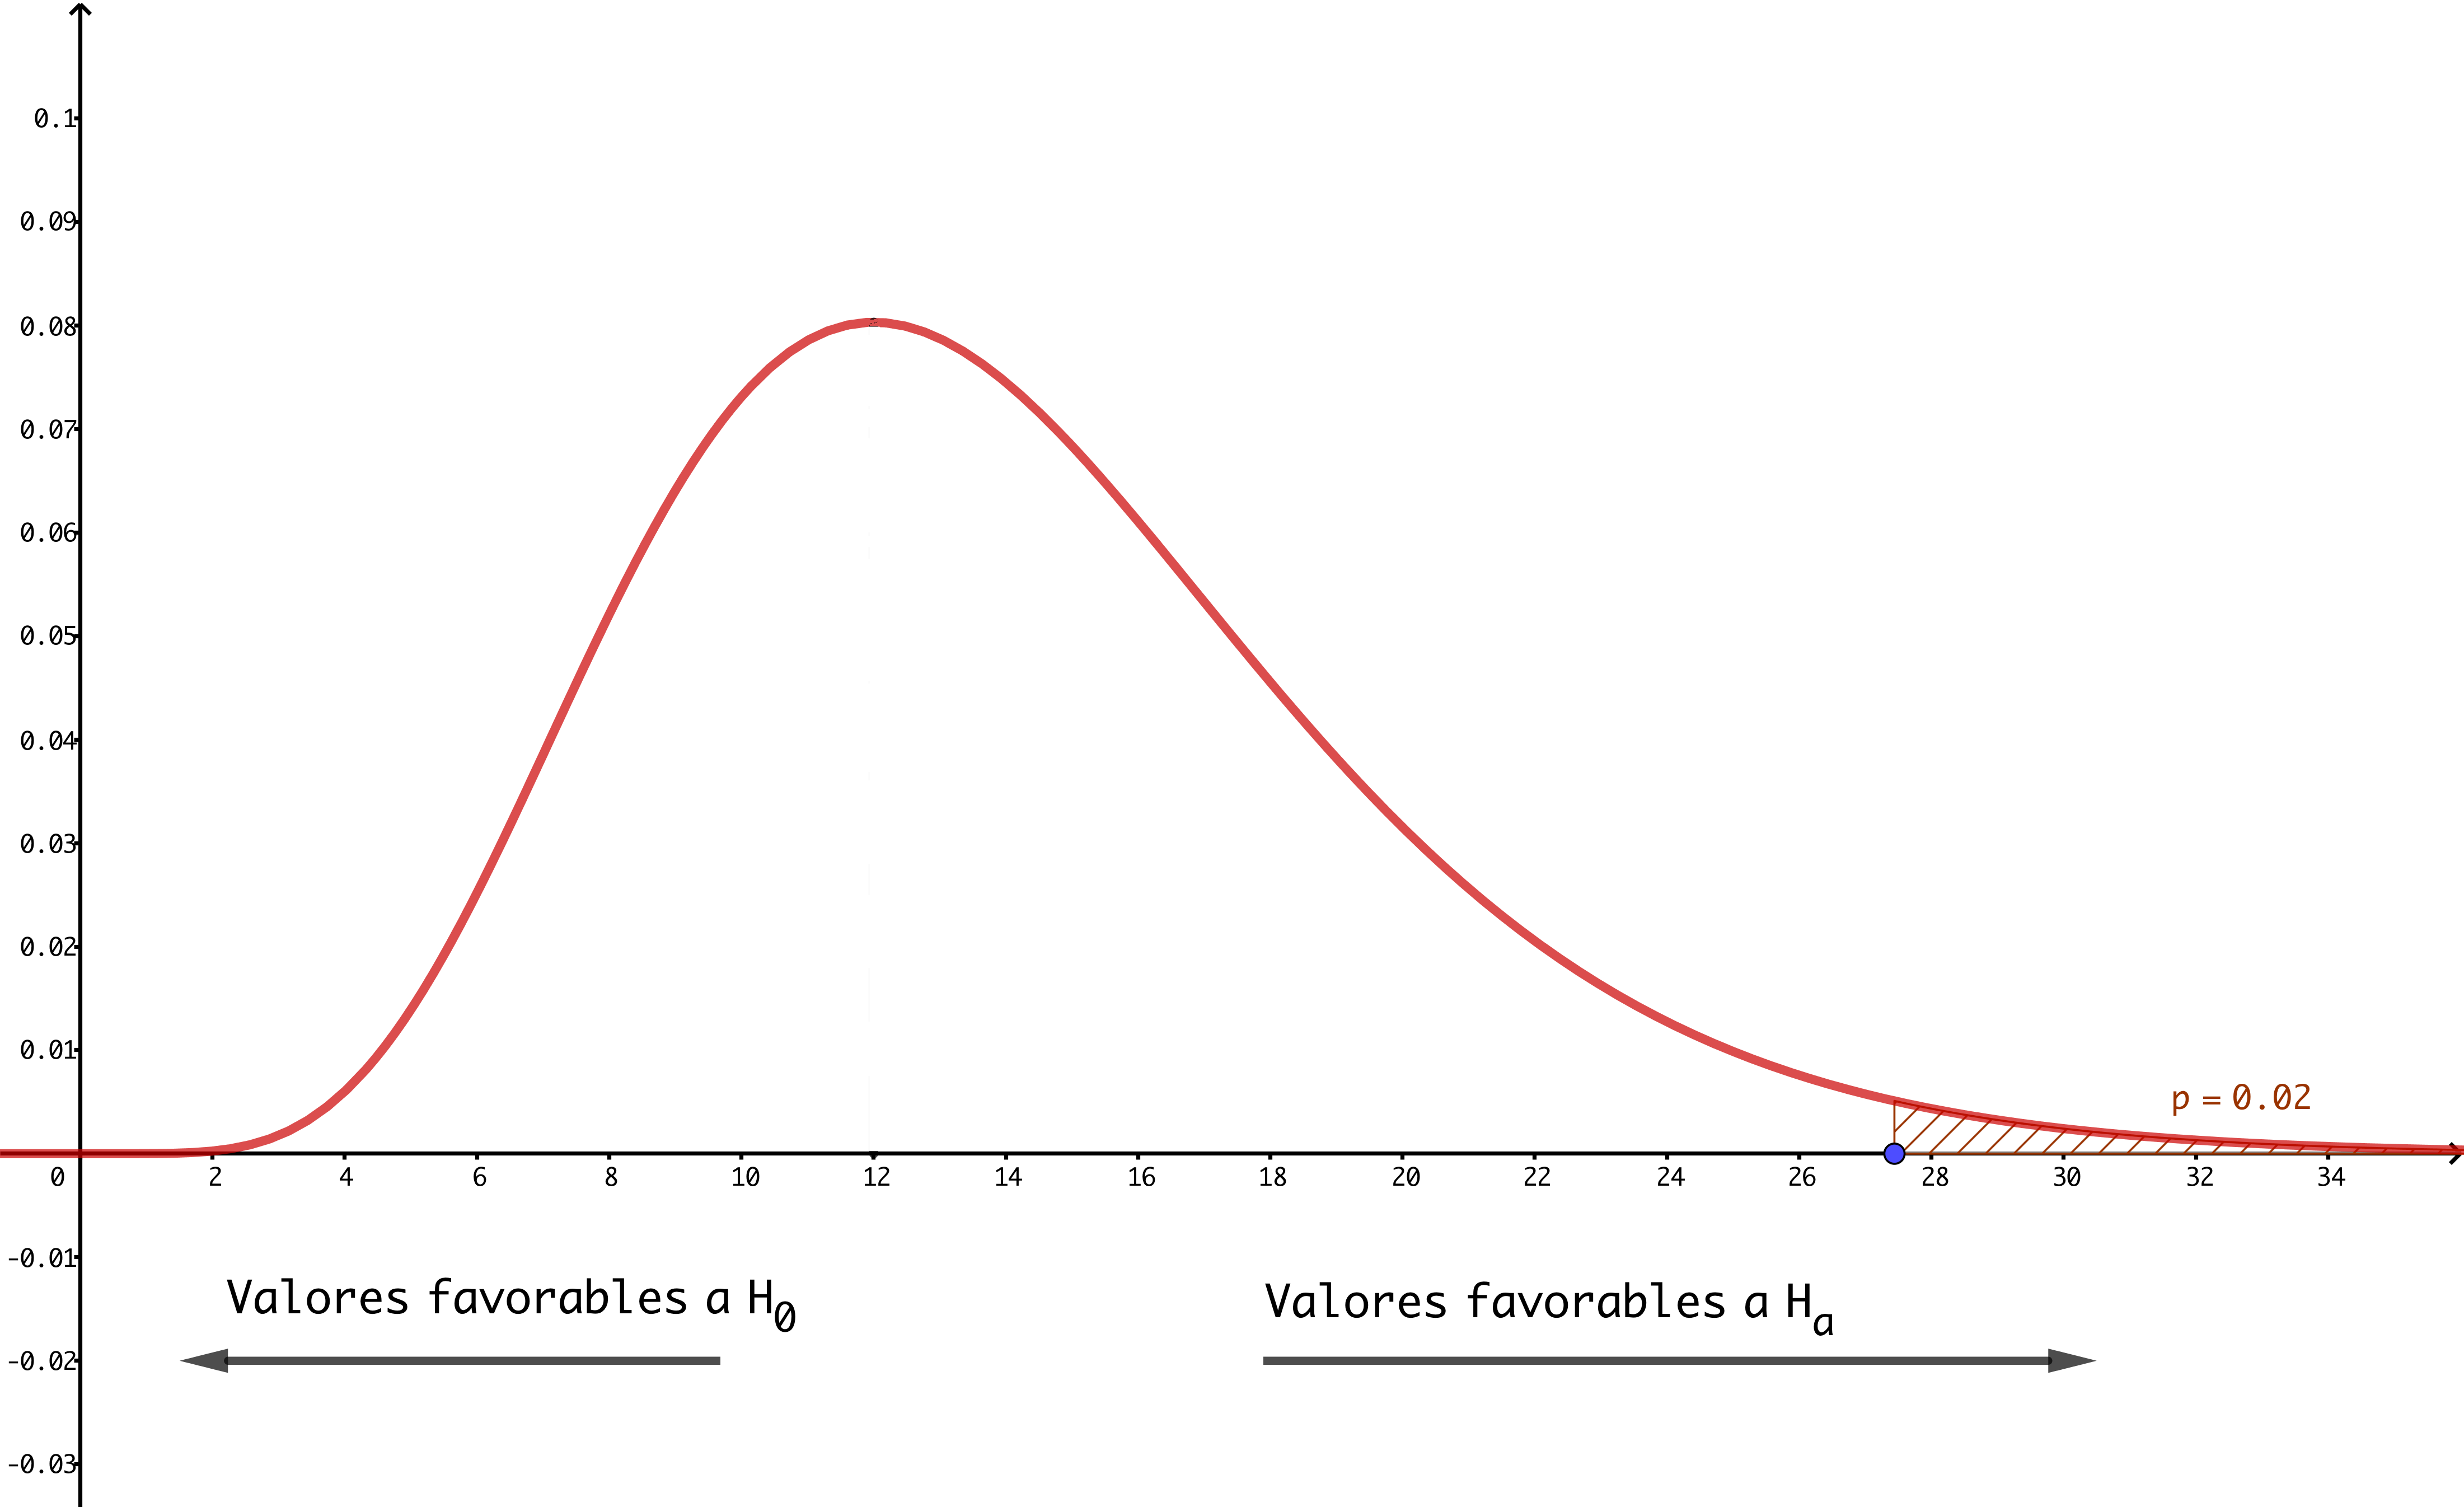
\includegraphics[width=8cm]{../fig/07-05-contrasteChi2} \end{center}

  Por tanto para obtener el p-valor calculamos la cola derecha: \[
  \text{ \tt pValor = 1 - pchisq(estadistico, df = n - 1)} \approx 0.01687
  \] con lo que a un nivel de significación del 95\% (\(\alpha = 0.05\))
  podemos rechazar \(H_0\) y concluir que los datos no permiten afirmar
  que la desviación típica sea menor o igual que \(0.5\).
\end{itemize}

\end{frame}

\begin{frame}[fragile]{Opcional: la función \texttt{sigma.test} de la
librería TeachingDemos.}
\protect\hypertarget{opcional-la-funcion-sigma.test-de-la-libreria-teachingdemos.}{}

\begin{itemize}
\item
  Aunque R básico no incluye ninguna función para los contrastes de
  varianza en una única variable normal, la librería TeachingDemos
  proporciona \texttt{sigma.test}. Asegúrate de instalarla antes de
  ejecutar este código que ilustra el contraste de
  \[H_a = \{\sigma^2 > 16\}\] en la variable \texttt{cty} de
  \texttt{mpg}.\small

\begin{Shaded}
\begin{Highlighting}[]
\KeywordTok{require}\NormalTok{(TeachingDemos)}
\end{Highlighting}
\end{Shaded}

\begin{verbatim}
## Loading required package: TeachingDemos
\end{verbatim}

\begin{Shaded}
\begin{Highlighting}[]
\NormalTok{(}\DataTypeTok{varTestCty =} \KeywordTok{sigma.test}\NormalTok{(mpg}\OperatorTok{$}\NormalTok{cty, }\DataTypeTok{sigmasq =} \DecValTok{16}\NormalTok{, }
           \DataTypeTok{alternative =} \StringTok{"greater"}\NormalTok{, }\DataTypeTok{conf.level =} \FloatTok{0.95}\NormalTok{))}
\end{Highlighting}
\end{Shaded}

\begin{verbatim}
## 
##    One sample Chi-squared test for variance
## 
## data:  mpg$cty
## X-squared = 263.77, df = 233, p-value = 0.0811
## alternative hypothesis: true variance is greater than 16
## 95 percent confidence interval:
##  15.65366      Inf
## sample estimates:
## var of mpg$cty 
##       18.11307
\end{verbatim}

  \normalsize
\end{itemize}

\end{frame}

\begin{frame}{Tamaño muestral y potencia del contraste.}
\protect\hypertarget{tamano-muestral-y-potencia-del-contraste.}{}

\begin{itemize}
\item
  Recordemos:\\
  \(-\) Error de tipo I: rechazar \(H_0\) cuando es cierta.
  \(P(\text{error tipo I}) = \alpha\).\\
  \(-\) Error de tipo II: rechazar \(H_a\) cuando es cierta.
  \(P(\text{error tipo II}) = \beta\).
\item
  La \textbf{potencia} de un contraste es \(1 -\beta\) y por tanto
  puedes pensar que:\small
  \[\mbox{potencia } =  1-\beta\, = \,1-P(\mbox{error de tipo II})  = \]
  \[
  = 1 - P(\mbox{rechazar }H_a | H_a\mbox{ es cierta}) = P(\mbox{rechazar }H_0 | H_0\mbox{ es falsa}).
  \] \normalsize
\item
  La potencia del contraste mide cómo de bueno es detectando una \(H_0\)
  falsa. En general nos gustaría tener a la vez \(\alpha\) pequeño y
  potencia grande. Pero, como en otros casos, no se pueden tener las dos
  cosas a la vez.
\item
  El cálculo de la potencia es en general complicado. \textbf{En el caso
  de un contraste para la media} es aproximadamente: \[
  \text{potencia} = 1 - \beta = K\, \dfrac{\delta\,\sqrt{n}\,\alpha}{\sigma}
  \] donde \(K\) es una constante de proporcionalidad, \(n\), \(\alpha\)
  y \(s\) son conocidos y \(\delta\) es el \textbf{tamaño del efecto}.
  Es decir, la diferencia mínima entre \(\mu\) y \(\mu_0\) que queremos
  que el contraste sea capaz de detectar para rechazar \(H_0\) en tal
  caso.
\end{itemize}

\end{frame}

\begin{frame}{Ecuaciones de potencia, observaciones generales}
\protect\hypertarget{ecuaciones-de-potencia-observaciones-generales}{}

\begin{itemize}
\item
  Observa la ecuación de potencia que hemos obtenido: \[
  \text{potencia} = 1 - \beta = K\, \dfrac{\delta\,\sqrt{n}\,\alpha}{\sigma}
  \]
\item
  Aunque esta ecuación es sencilla, ilustra varias ideas importantes
  sobre la potencia:

  \(1\). \(n\) es el tamaño de la muestra. A más muestra, más potencia.

  \(2\). \(\delta\) es la diferencia entre \(\mu\) y \(\mu_0\). Es
  decir, el \emph{efecto} que esperamos detectar. Cuanto mayor sea el
  efecto, mayor potencia.

  \(3\). \(\alpha\) es el nivel de significación del contraste, que
  solemos fijar en \(0.05\). \textbf{No podemos tener a la vez
  \(\alpha\) pequeño y potencia = \(1 - \beta\) grande}

  \(4.\) \(\sigma\) es la desviación típica, que indica la dispersión de
  la población. La solemos estimar con \(s\), a menudo procedente de
  estudios piloto o previos. Y a mayor dispersión, menor potencia.
\end{itemize}

\end{frame}

\begin{frame}{Curvas de potencia.}
\protect\hypertarget{curvas-de-potencia.}{}

\begin{itemize}
\item
  Las ecuaciones de potencia permiten dibujar las llamadas \emph{curvas
  de potencia} que, para valores de \(n\), \(\alpha\) y \(s\) fijos,
  muestran como depende la potencia del tamaño del efecto (medido en
  ``unidades'' \(s\)). El aspecto típico de una de estas curvas es:

  \begin{center}\includegraphics[width=0.5\linewidth]{05-IntroduccionInferencia_files/figure-beamer/unnamed-chunk-40-1} \end{center}

  que confirma la idea de que a mayor tamaño del efecto, mayor es la
  potencia.
\end{itemize}

\end{frame}

\begin{frame}[fragile]{La función power.t.test}
\protect\hypertarget{la-funcion-power.t.test}{}

\begin{itemize}
\item
  Las ecuaciones de potencia permiten determinar el tamaño muestral
  necesario para poder detectar un efecto de tamaño dado, con niveles de
  significación y potencia dados. En R las funciones con nombres que
  empiezan por power sirven para esto.
\item
  \textbf{Ejemplo:} ¿Cuál es el tamaño muestral \(n\) necesario para un
  contraste unilateral de hipótesis con \(nc = 0.99\)
  (\(\alpha = 0.01\)) y potencia \(1 - \beta = 0.80\) que sea capaz de
  detectar un efecto (diferencia entre las medias \(\mu\) y \(\mu_0\))
  mayor o igual a \(\delta = 0.1\)? En un estudio piloto obtuvimos
  \(s = 0.5\).
\item
  Usamos:\scriptsize

\begin{Shaded}
\begin{Highlighting}[]
\KeywordTok{power.t.test}\NormalTok{(}\DataTypeTok{delta =} \FloatTok{0.1}\NormalTok{, }\DataTypeTok{sd =} \FloatTok{0.5}\NormalTok{, }\DataTypeTok{sig.level =} \FloatTok{0.05}\NormalTok{,}
             \DataTypeTok{power =} \FloatTok{0.80}\NormalTok{, }\DataTypeTok{type=}\StringTok{"one.sample"}\NormalTok{, }\DataTypeTok{alternative=}\StringTok{"one.sided"}\NormalTok{)}
\end{Highlighting}
\end{Shaded}

\begin{verbatim}
## 
##      One-sample t test power calculation 
## 
##               n = 155.9257
##           delta = 0.1
##              sd = 0.5
##       sig.level = 0.05
##           power = 0.8
##     alternative = one.sided
\end{verbatim}

  \normalsize
\item
  \textbf{Ejercicio.} Aquí hemos calculado \(n\), pero esta función
  puede usarse para determinar uno de los valores a partir de los
  restantes. Prueba \scriptsize

\begin{verbatim}
power.t.test(delta = 0.1, sd = 0.5, sig.level = 0.05, n = 300, 
             type="one.sample", alternative="one.sided")
\end{verbatim}

  \normalsize
\end{itemize}

\end{frame}

\hypertarget{uso-y-abuso-del-p-valor.}{%
\section{Uso y abuso del p-valor.}\label{uso-y-abuso-del-p-valor.}}

\begin{frame}

\begin{center}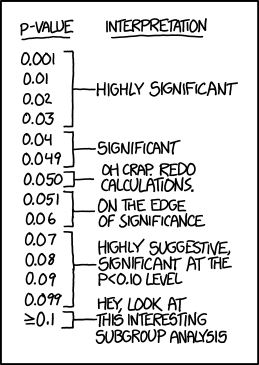
\includegraphics[width=0.5\linewidth]{../fig/xkcd_p_values_2x} \end{center}

\end{frame}

\begin{frame}{Significación estadística vs relevancia científica.}
\protect\hypertarget{significacion-estadistica-vs-relevancia-cientifica.}{}

\begin{itemize}
\item
  \emph{Un fabricante garantiza que produce comprimidos de diámetro
  medio de 13mm. En una muestra de 50 unidades tiene un diámetro medio
  \(\bar X =13.05\)mm, desviación típica \(s = 0.6\)mm. ¿Es aceptable
  esta afirmación al nivel de significación del 99\%?}
\item
  La hipótesis nula es \(H_0:\{\mu = 13\}\), y la alternativa
  \(H_a:\{\mu\neq 13\}\). El estadístico y p-valor (calculado con la
  \(t\) de Student) son: \[
  T = \dfrac{\bar X - \mu_0}{\frac{s}{\sqrt{n}}} =
  \dfrac{13.05 - 13}{\frac{0.6}{\sqrt{50}}}\approx
  0.5893,\qquad
  \text{p-valor: }
  0.5584
  \]
\item
  El contraste \textbf{no} es significativo, rechazamos \(H_a\). Fíjate
  en que el efecto es \(\delta = 0.05\). Pero ahora repetimos la cuenta
  con los mismos valores, salvo que aumentamos el tamaño muestral a
  \(n = 5000\).
\end{itemize}

\[
T = \dfrac{\bar X - \mu_0}{\frac{s}{\sqrt{n}}} =
\dfrac{13.05 - 13}{\frac{0.6}{\sqrt{5000}}}\approx
5.893,\qquad
\text{p-valor: }
\ensuremath{4.052\times 10^{-9}}
\]

\begin{itemize}
\tightlist
\item
  Ahora el p-valor es \emph{muy} pequeño y rechazamos \(H_0\). Este
  ejemplo ilustra un principio general: \textbf{si se usan muestras
  suficientemente grandes, incluso un efecto \(\delta = \mu - \mu_0\)
  muy pequeño (irrelevante) puede llegar a ser estadísticamente
  significativo.}
\end{itemize}

\end{frame}

\begin{frame}{Relevancia y la d de Cohen.}
\protect\hypertarget{relevancia-y-la-d-de-cohen.}{}

\begin{itemize}
\item
  ¿Como podemos entonces juzgar la \textbf{relevancia} del efecto
  observado? El primer consejo es que \emph{los resultados de un
  contraste deberían ir siempre acompañados de estimaciones del tamaño
  del efecto}. Por ejemplo, usando intervalos de confianza.
\item
  La \textbf{d de Cohen} es: \[d = \dfrac{\bar X - \mu_0}{s}\] Podemos
  usarla para hacernos una idea aproximada de la relevancia del efecto
  observado teniendo en cuenta estas indicaciones:

  \(-\) Un valor \(d < 0.2\) indica un efecto no relevante.\\
  \(-\) Si es \(d > 0.8\) es muy posible que la diferencia sea
  relevante. \(-\) Cuando \(0.2 < d < 0.8\) se necesita la
  \textbf{opinión de un experto} que juzgue la relevancia de los
  resultados.
\item
  En el ejemplo anterior, con la muestra grande, se obtiene:

  \[
  d = \dfrac{\bar X - \mu_0}{s} =
  \dfrac{13.05 - 13}{0.6}\approx
  0.08333
  \] así que parece que ese efecto \(\delta = 0.05\) es, seguramente,
  irrelevante.
\end{itemize}

\end{frame}

\hypertarget{uso-y-abuso-del-p-valor.-1}{%
\section{Uso y abuso del p-valor.}\label{uso-y-abuso-del-p-valor.-1}}

\begin{frame}[fragile]{El problema de los contrastes múltiples.}
\protect\hypertarget{el-problema-de-los-contrastes-multiples.}{}

\begin{itemize}
\item
  El contraste de hipótesis es el método habitual para confirmar un
  resultado científico o técnico a partir de los datos. Pero su uso
  puede prestarse a errores o incluso a manipulaciones mal
  intencionadas.
\item
  Por ejemplo, ya sabemos que \(\alpha\) es la probabilidad de cometer
  un error de tipo I (rechazar una \(H_0\) cierta). Si por ejemplo
  \(\alpha = 0.05\). Si realizamos 20 contrastes independientes de
  hipótesis nulas \textbf{todas ellas ciertas} ¿cuál es la probabilidad
  de que (nos toque alguna muestra mala y) rechacemos alguna \(H_0\)? Es
  fácil ver que la situación tiene todos los ingredientes de una
  binomial \(B(20, \alpha)\) y si \(X = (\)número de \(H_0\) rechazadas)
  entonces
  \[P(X > 0) = 1 - P(X = 0) = 1 - (1 - \alpha)^{20}\approx0.641514\] que
  también puedes calcular en R como:
  \texttt{1\ -\ dbinom(0,\ size\ =\ 20,\ prob\ =\ 0.05)}.
\item
  Eso significa que simplemente repitiendo el contraste 20 veces hay un
  64\% de probabilidades de obtener un resultado \emph{significativo ¡¡y
  falso!!}.
\end{itemize}

\end{frame}

\begin{frame}[fragile]{Simulando contrastes múltiples con R.}
\protect\hypertarget{simulando-contrastes-multiples-con-r.}{}

\begin{itemize}
\item
  Vamos a usar R para confirmar la discusión anterior en una
  simulación.\small

\begin{Shaded}
\begin{Highlighting}[]
\KeywordTok{set.seed}\NormalTok{(}\DecValTok{2019}\NormalTok{)}
\NormalTok{nTests =}\StringTok{ }\DecValTok{20} \CommentTok{# Haremos 20 contrastes}
\CommentTok{# y este vector los 20 p-valores}
\NormalTok{pValores =}\StringTok{ }\KeywordTok{numeric}\NormalTok{(nTests)}
\CommentTok{# Ahora hacemos los contrastes y guardamos los p-valores}
\ControlFlowTok{for}\NormalTok{(i }\ControlFlowTok{in} \DecValTok{1}\OperatorTok{:}\NormalTok{nTests)\{}
\NormalTok{  muestra =}\StringTok{ }\KeywordTok{c}\NormalTok{(}\KeywordTok{rnorm}\NormalTok{(}\DecValTok{15}\NormalTok{))}
\NormalTok{  pValores[i] =}\StringTok{ }\KeywordTok{t.test}\NormalTok{(muestra, }\DataTypeTok{alternative =} \StringTok{"two.sided"}\NormalTok{, }\DataTypeTok{mu =} \DecValTok{0}\NormalTok{)}\OperatorTok{$}\NormalTok{p.value}
\NormalTok{\}}
\CommentTok{# ¿Cuál es el p-valor más pequeño?}
\KeywordTok{min}\NormalTok{(pValores)}
\end{Highlighting}
\end{Shaded}

\begin{verbatim}
## [1] 0.03307146
\end{verbatim}

  \normalsize Como puede verse, hay al menos un p-valor \(< \alpha\),
  así que estaríamos rechazando incorrectamente al menos una de las
  \(H_0\).
\item
  Una primera solución consiste en aplicar la
  \link{https://en.wikipedia.org/wiki/Bonferroni_correction}{corrección de Bonferroni},
  que en esencia cambia el criterio de rechazo de \(H_0\) de p-valor
  \(< \alpha\) por el criterio p-valor \(< \frac{\alpha}{m}\) siendo
  \(m\) el número de contrastes.
\end{itemize}

\end{frame}

\begin{frame}

\begin{center}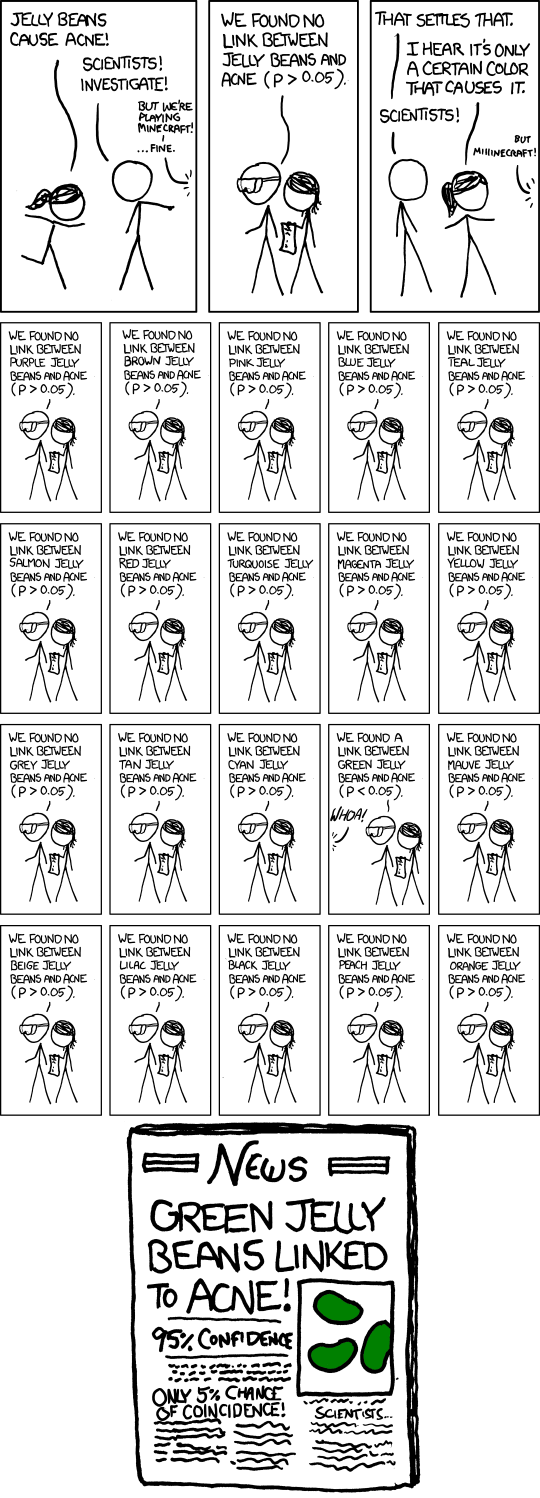
\includegraphics[width=0.5\linewidth]{../fig/xkcd_Significant} \end{center}

\href{https://xkcd.com/882/}{XKCD}

\end{frame}

\begin{frame}{p-hacking y otras problemáticas.}
\protect\hypertarget{p-hacking-y-otras-problematicas.}{}

\begin{itemize}
\item
  La situación que acabamos de describir puede ocurrir por
  desconocimiento, pero también puede ser una estratagema de alguien
  tratando de obtener un resultado significativo a cualquier coste. Este
  tipo de manejos forman parte de lo que se denomina
  \link{https://en.wikipedia.org/wiki/Data_dredging}{p-hacking, o data-dredging}.
\item
  Recomendamos leer esta nota breve de
  \href{http://www.investigacionyciencia.es/noticias/grandes-expertos-en-el-uso-de-la-estadstica-proclaman-que-0-05-no-es-el-filtro-adecuado-15521?utm_source=boletin\&utm_medium=email\&utm_campaign=Del+1+al+8+de+septiembre}{\textcolor{blue}{Investigación y Ciencia}}
  o aún mejor el
  \href{https://www.nature.com/news/big-names-in-statistics-want-to-shake-up-much-maligned-p-value-1.22375}{\textcolor{blue}{artículo de Nature}}
  del que procede, o este
  \href{http://www.nature.com/news/scientific-method-statistical-errors-1.14700}{\textcolor{blue}{otro más extenso}},
  de Regina Nuzzo, también en Nature.
\item
  El control del error en contrastes repetidos es un tema ha sido objeto
  de estudio intenso recientemente. Por ejemplo en \emph{Genómica} o en
  \emph{Big Data} son comunes los casos en los que se contrastan decenas
  de miles de hipótesis a la vez (uno por gen, por ejemplo). En esos
  casos usar correcciones tipo Bonferroni sería demasiado drástico:
  rechazaríamos demasiado pocas \(H_0\). Una referencia elemental para
  empezar a entender este tema es
  \link{https://en.wikipedia.org/wiki/Family-wise_error_rate}{este artículo}
  dela Wikipedia.
\end{itemize}

\end{frame}

\hypertarget{complementos-de-r.}{%
\section{Complementos de R.}\label{complementos-de-r.}}

\begin{frame}[fragile]{Listas.}
\protect\hypertarget{listas.}{}

\begin{itemize}
\item
  Como referencias para este apartado puedes usar (Boehmke 2016,
  capítulo 11), (Matloff 2011, capítulo 4).
\item
  A diferencia de los vectores, las listas sirven para guardar elementos
  heterogéneos (incluidas sublistas). La forma más sencilla de crear una
  lista es usando \texttt{list}:\small

\begin{Shaded}
\begin{Highlighting}[]
\NormalTok{(}\DataTypeTok{planeta =} \KeywordTok{list}\NormalTok{(}\DataTypeTok{nombre =} \StringTok{"Marte"}\NormalTok{, }\DataTypeTok{exterior =} \OtherTok{TRUE}\NormalTok{, }
                 \DataTypeTok{radio =} \FloatTok{3389.5}\NormalTok{, }\DataTypeTok{satelites =} \KeywordTok{list}\NormalTok{(}\StringTok{"Fobos"}\NormalTok{, }\StringTok{"Deimos"}\NormalTok{)))}
\end{Highlighting}
\end{Shaded}

\begin{verbatim}
## $nombre
## [1] "Marte"
## 
## $exterior
## [1] TRUE
## 
## $radio
## [1] 3389.5
## 
## $satelites
## $satelites[[1]]
## [1] "Fobos"
## 
## $satelites[[2]]
## [1] "Deimos"
\end{verbatim}

  \normalsize
\end{itemize}

\end{frame}

\begin{frame}[fragile]{Accediendo a los elementos de una lista.}
\protect\hypertarget{accediendo-a-los-elementos-de-una-lista.}{}

\begin{itemize}
\item
  R usa \texttt{\$} o doble corchete \texttt{{[}{[}\ {]}{]}} para
  identificar los elementos de la lista.\small

\begin{Shaded}
\begin{Highlighting}[]
\NormalTok{planeta[[}\DecValTok{1}\NormalTok{]]}
\end{Highlighting}
\end{Shaded}

\begin{verbatim}
## [1] "Marte"
\end{verbatim}

\begin{Shaded}
\begin{Highlighting}[]
\NormalTok{planeta}\OperatorTok{$}\NormalTok{exterior}
\end{Highlighting}
\end{Shaded}

\begin{verbatim}
## [1] TRUE
\end{verbatim}

\begin{Shaded}
\begin{Highlighting}[]
\NormalTok{planeta}\OperatorTok{$}\NormalTok{satelites[[}\DecValTok{1}\NormalTok{]]}
\end{Highlighting}
\end{Shaded}

\begin{verbatim}
## [1] "Fobos"
\end{verbatim}

  \normalsize La salida es del tipo de objeto que hay en esa posición de
  la lista.
\item
  Pero fíjate en la diferencia si usamos un único corchete:\small

\begin{Shaded}
\begin{Highlighting}[]
\NormalTok{planeta[}\DecValTok{1}\NormalTok{]}
\end{Highlighting}
\end{Shaded}

\begin{verbatim}
## $nombre
## [1] "Marte"
\end{verbatim}

\begin{Shaded}
\begin{Highlighting}[]
\NormalTok{planeta[}\StringTok{"exterior"}\NormalTok{]}
\end{Highlighting}
\end{Shaded}

\begin{verbatim}
## $exterior
## [1] TRUE
\end{verbatim}

  \normalsize En este caso la salida \emph{siempre es una lista}.
\end{itemize}

\end{frame}

\begin{frame}[fragile]{Funciones \texttt{list}, \texttt{append} y
\texttt{c}.}
\protect\hypertarget{funciones-list-append-y-c.}{}

\begin{itemize}
\item
  Atención a esta diferencia:\scriptsize

\begin{Shaded}
\begin{Highlighting}[]
\NormalTok{(}\DataTypeTok{l1 =} \KeywordTok{list}\NormalTok{(}\StringTok{"A"}\NormalTok{, }\StringTok{"B"}\NormalTok{))}
\end{Highlighting}
\end{Shaded}

\begin{verbatim}
## [[1]]
## [1] "A"
## 
## [[2]]
## [1] "B"
\end{verbatim}

\begin{Shaded}
\begin{Highlighting}[]
\NormalTok{(}\DataTypeTok{l2 =} \KeywordTok{list}\NormalTok{(}\KeywordTok{c}\NormalTok{(}\StringTok{"A"}\NormalTok{, }\StringTok{"B"}\NormalTok{)))}
\end{Highlighting}
\end{Shaded}

\begin{verbatim}
## [[1]]
## [1] "A" "B"
\end{verbatim}

  \normalsize La función \texttt{list} siempre crea \emph{listas
  anidadas}. Por ejemplo este comando (no se muestra la salida) crea una
  lista con dos componentes y el primero es \texttt{l2}:\scriptsize

\begin{Shaded}
\begin{Highlighting}[]
\NormalTok{(}\DataTypeTok{l3 =} \KeywordTok{list}\NormalTok{(l2, }\StringTok{"C"}\NormalTok{))}
\end{Highlighting}
\end{Shaded}

  \normalsize
\item
  Las funciones \texttt{append} y \texttt{c} \emph{adjuntan} elementos.
  Estos comandos son equivalentes:\scriptsize

\begin{Shaded}
\begin{Highlighting}[]
\NormalTok{l4 =}\StringTok{ }\KeywordTok{append}\NormalTok{(l2, }\StringTok{"D"}\NormalTok{)}
\NormalTok{(}\DataTypeTok{l4 =} \KeywordTok{c}\NormalTok{(l2, }\StringTok{"D"}\NormalTok{))}
\end{Highlighting}
\end{Shaded}

\begin{verbatim}
## [[1]]
## [1] "A" "B"
## 
## [[2]]
## [1] "D"
\end{verbatim}

  \normalsize También se pueden añadir elementos por nombre, como en\\
  \small \texttt{planeta\$distSol\ =\ 227.9} \normalsize 
\end{itemize}

\end{frame}

\begin{frame}[fragile]{Otras propiedades y operaciones con listas.}
\protect\hypertarget{otras-propiedades-y-operaciones-con-listas.}{}

\begin{itemize}
\item
  La función \texttt{length} produce el número de elementos de una
  lista. Y con \texttt{names} se obtienen los nombres de sus elementos
  (si se han dado nombres).
\item
  \textbf{Ejercicio:} Prueba a usar \texttt{names} y \texttt{length} con
  varias de las listas que hemos creado. Ejecuta
  \texttt{(sesion\ =\ sessionInfo())}
  \texttt{para\ ver\ lo\ que\ hace\ esa\ función.\ Y\ luego\ explora\ como\ acceder\ a\ las\ componentes\ usando}sesion\$`
\item
  Para eliminar elementos de una lista basta con hacerlos
  \texttt{NULL}.\small

\begin{Shaded}
\begin{Highlighting}[]
\NormalTok{l4[}\DecValTok{3}\NormalTok{] =}\StringTok{ }\OtherTok{NULL}
\NormalTok{l4}
\end{Highlighting}
\end{Shaded}

\begin{verbatim}
## [[1]]
## [1] "A" "B"
## 
## [[2]]
## [1] "D"
\end{verbatim}

  \normalsize
\item
  La función \texttt{unlist} \emph{\texttt{aplana}} una lista dando como
  resultado un vector:\small

\begin{Shaded}
\begin{Highlighting}[]
\KeywordTok{unlist}\NormalTok{(l1)}
\end{Highlighting}
\end{Shaded}

\begin{verbatim}
## [1] "A" "B"
\end{verbatim}

  \normalsize
\item
  \textbf{Ejercicio:} ¿qué se obtiene al aplicar \texttt{unlist} a la
  siguiente \texttt{lista}?\\
  \small \texttt{lista\ =\ list(letters{[}1:3{]},\ matrix(1:12,\ nrow\ =\ 3),\ TRUE)}.
  \normalsize
\end{itemize}

\end{frame}

\begin{frame}[fragile]{Estructuras de control en R. Bloques if/else.}
\protect\hypertarget{estructuras-de-control-en-r.-bloques-ifelse.}{}

\begin{itemize}
\item
  Como referencias para este apartado puedes usar (Boehmke 2016,
  capítulo 19), (Matloff 2011, capítulo 7).
\item
  \textbf{Bloques if/else.} La estructura básica de estos bloques
  es:\small

\begin{verbatim}
if (condición) {
  ...
  sentencias que se ejecutan si condicion = TRUE
  ...
}  else {
  ...
  sentencias que se ejecutan si condicion = FALSE
  ...
}
\end{verbatim}

  \normalsize Si necesitas condiciones anidadas puedes cambiar
  \texttt{else} por \texttt{else\ if} y añadir a continuación otra
  condición para crear un nuevo nivel de la estructura.
\item
  La estructura \texttt{if} está pensada para ejecutarse sobre una
  \emph{única} condición que produzca un \emph{único} valor
  \texttt{TRUE/FALSE}. Existe también una función vectorializada,
  llamada \texttt{ifelse} que se puede aplicar a un vector de
  condiciones. Un ejemplo:\small

\begin{Shaded}
\begin{Highlighting}[]
\KeywordTok{ifelse}\NormalTok{(((}\DecValTok{1}\OperatorTok{:}\DecValTok{5}\NormalTok{) }\OperatorTok{<}\StringTok{ }\DecValTok{3}\NormalTok{), }\DataTypeTok{yes =} \StringTok{"A"}\NormalTok{,  }\DataTypeTok{no =} \StringTok{"B"}\NormalTok{)}
\end{Highlighting}
\end{Shaded}

\begin{verbatim}
## [1] "A" "A" "B" "B" "B"
\end{verbatim}

  \normalsize
\end{itemize}

\end{frame}

\begin{frame}[fragile]{Bucles for.}
\protect\hypertarget{bucles-for.}{}

\begin{itemize}
\item
  El bucle for se utiliza cuando queremos repetir un bloque de comando y
  conocemos de antemano el número máximo de repeticiones. Su estructura
  básica es similar a esta:\small

\begin{verbatim}
for(k in valores_k) {
  ...
  cuerpo del bucle, se repite a lo sumo length(valores_k) veces
  ...
}
\end{verbatim}

  \normalsize La variable \texttt{k} (el nombre es arbitrario) es el
  \emph{contador} del bucle for. El vector \texttt{valores\_k} contiene
  los valores que toma \texttt{k} en cada iteración.
\item
  Si en alguna iteración queremos interrumpir el bucle cuando se cumple
  alguna condición (y no hacer ninguna iteración más), podemos combinar
  \texttt{if} con la función \texttt{break}. Si lo que queremos es
  solamente pasar a la siguiente iteración usamos \texttt{next} en lugar
  de \texttt{break}.
\item
  A menudo se usa un bucle for para \emph{``rellenar''} un objeto como
  un vector o matriz. Es importante recordar que R es poco eficiente
  haciendo \emph{``crecer''} estos objetos. En esos casos es mucho mejor
  comenzar creando el objeto completo, con todas sus posiciones, e ir
  asignado valores a posiciones en cada iteración (R lo inicializa a 0
  ).
\item
  En general \textbf{es preferible usar operaciones vectorializadas en
  lugar de bucles for}. Pronto aprenderemos las funciones de la familia
  \texttt{apply} para hacer esto.
\end{itemize}

\end{frame}

\begin{frame}[fragile]{Ejemplo de bucle for con \texttt{next} y
\texttt{break}.}
\protect\hypertarget{ejemplo-de-bucle-for-con-next-y-break.}{}

\begin{itemize}
\item
  El siguiente código ilustra un bucle for con el uso de next y break.
  Ejecútalo varias veces para ver como se comporta según los valores de
  sus parámetros.

\begin{Shaded}
\begin{Highlighting}[]
\NormalTok{valores =}\StringTok{ }\KeywordTok{numeric}\NormalTok{(}\DecValTok{10}\NormalTok{) }\CommentTok{# Creamos un vector del tamaño previsto}
\ControlFlowTok{for}\NormalTok{ (k }\ControlFlowTok{in} \DecValTok{1}\OperatorTok{:}\DecValTok{10}\NormalTok{)\{}
\NormalTok{  sorteo =}\StringTok{ }\KeywordTok{sample}\NormalTok{(}\DecValTok{1}\OperatorTok{:}\DecValTok{20}\NormalTok{, }\DecValTok{1}\NormalTok{)}
  \KeywordTok{print}\NormalTok{(}\KeywordTok{paste0}\NormalTok{(}\StringTok{"k = "}\NormalTok{, k, }\StringTok{", sorteo = "}\NormalTok{, sorteo))}
  \ControlFlowTok{if}\NormalTok{ (k }\OperatorTok\StringTok{ }\DecValTok{5}\OperatorTok{:}\DecValTok{6}\NormalTok{)\{}
    \ControlFlowTok{next} \CommentTok{# saltamos dos valores}
\NormalTok{  \} }\ControlFlowTok{else} \ControlFlowTok{if}\NormalTok{ (sorteo  }\OperatorTok{==}\StringTok{ }\DecValTok{1}\NormalTok{)\{}
    \KeywordTok{print}\NormalTok{(}\StringTok{"Resultado del sorteo es 1, fin del bucle"}\NormalTok{)}
    \ControlFlowTok{break} \CommentTok{# paramos si un valor aleatorio es 1}
\NormalTok{  \}}
\NormalTok{  valores[k] =}\StringTok{ }\NormalTok{k }\CommentTok{# se ejecuta cuando no se cumplan las condiciones}
\NormalTok{\} }
\NormalTok{valores}
\end{Highlighting}
\end{Shaded}
\item
  \textbf{Ejercicio:} ¿Qué valores asigna R a los elementos de los
  vectores creados respectivamente con \texttt{x\ =\ logical(10)} y con
  \texttt{v\ =\ character(10)}?
\end{itemize}

\end{frame}

\begin{frame}[fragile]{Otros bucles: while y repeat.}
\protect\hypertarget{otros-bucles-while-y-repeat.}{}

\begin{itemize}
\item
  En R también existen estos dos tipos de bucles, comunes a muchos
  lenguajes. Conviene insistir en que suele ser más eficiente evitar el
  uso de bucles.
\item
  El bucle \texttt{while} tiene esta estructura:\small

\begin{verbatim}
while (condición){
    ...
    cuerpo del bucle, que eventualmente debe hacer condición TRUE o usar break
    ...
}
\end{verbatim}

  \normalsize
\item
  El bucle \texttt{repeat} tiene esta estructura:\small

\begin{verbatim}
repeat {
    ...
    cuerpo del bucle, que debe usar break
    ...
}
\end{verbatim}

  \normalsize Insistimos: a diferencia de otros lenguajes, en R un bucle
  \texttt{repeat} debe usar explícitamente \texttt{break} para
  detenerse.
\item
  El código de este tema contiene ejemplos de bucle \texttt{while} y
  \texttt{repeat} con \texttt{break}, que puedes ejecutar varias veces.
  Observa las diferencias en el comportamiento de ambos bucles.
\end{itemize}

\end{frame}

\begin{frame}{Rmarkdown para la creación de documentos.}
\protect\hypertarget{rmarkdown-para-la-creacion-de-documentos.}{}

\begin{itemize}
\item
  En las sesiones del curso veremos algunos ejemplos sencillos para que
  puedas iniciarte en el manejo de Rmarkdown.
\item
  Rmarkdown, creado por Yihui Xie, es una herramienta muy general para
  la creación de documentos, en especial documentos relacionados con el
  Análisis de Datos. A partir de los ficheros escritos con Rmarkdown se
  pueden obtener fácilmente salidas en formato pdf o HTML, pero también
  presentaciones, artículos e informes técnicos, entradas de blog,
  libros, dashboards con Shiny y la lista sigue creciendo.
\item
  Hay dos fuentes de información online básicas para adentrarse en las
  posibilidades de RMarkdown:\\
  Del propio Yihui Xie:
  \link{https://bookdown.org/yihui/rmarkdown/}{R Markdown: The Definitive Guide.}\\
  De RStudio:
  \link{https://rmarkdown.rstudio.com/lesson-1.html}{R Markdown: Get Started.}
\item
  Recomendamos empezar leyendo una
  \link{http://www.unavarra.es/personal/tgoicoa/ESTADISTICA_RMarkdown_tomas/basicRmarkdown/index.html}{introducción recciente a RMarkdon}
  de T. Goicoa (Univ. Pública de Navarra).
\end{itemize}

\end{frame}

\begin{frame}{Referencias para la sesión}
\protect\hypertarget{referencias-para-la-sesion}{}

\textbf{Enlaces}

\begin{itemize}
\item
  \link{https://raw.githubusercontent.com/fernandosansegundo/MBDFME/master/scripts/05- InferenciaMediaUnaVariable.R}{Código de esta sesión}
\end{itemize}

\textbf{Bibliografía}

\hypertarget{refs}{}
\leavevmode\hypertarget{ref-Boehmke2016}{}%
Boehmke, Bradley C. 2016. \emph{Data Wrangling with R}. Springer.
\url{https://doi.org/10.1007/978-3-319-45599-0}.

\leavevmode\hypertarget{ref-crawley2005statistics}{}%
Crawley, Michael J. 2005. \emph{Statistics: an introduction using R. 327
p}. John Wiley Sons.

\leavevmode\hypertarget{ref-Matloff2011}{}%
Matloff, Norman S. 2011. \emph{The art of R programming : tour of
statistical software design}. No Starch Press.
\url{https://doi.org/10.1080/09332480.2012.685374}.

\end{frame}

\end{document}
